\documentclass[11pt]{article}
\usepackage[utf8]{inputenc}
\usepackage[T1]{fontenc}
\usepackage{lmodern}
\usepackage{graphicx} % Required for inserting images
\usepackage{hyperref}
\usepackage{picture}
\usepackage{graphics}
\usepackage{float}
\usepackage{microtype}
\usepackage[a4paper, margin=1in]{geometry}
\usepackage[slovak]{babel}
\usepackage{parskip}

\begin{document}
\begin{titlepage}
    \begin{center}

        {\Large \textbf{Slovenská technická univerzita v Bratislave}}\\[0.3cm]
        {\large Fakulta informatiky a informačných technológií}\\[7cm]

        {\Huge \textbf{IA-TARA}}\\[0.5cm]
        {\Large Týmový projekt}\\[10cm]

        \begin{flushleft}
            \large
            Autori:\\
            \textbf{Bc. Marko Šebest} \\
            \textbf{Bc. Samuel Švenk} \\
            \textbf{Bc. Oliver Nemček} \\
            \textbf{Bc. Richard Blažo} \\
            \textbf{Bc. Danylo Tokarskyi} \\
            \textbf{Bc. Martin Čulen} \\
        \end{flushleft}

        \vfill

        {\large Bratislava \hfill 2025/26}

    \end{center}
\end{titlepage}

\tableofcontents
\newpage

\section{Úvod}
\textbf{TARA (Threat Analysis and Risk Assessment)} je systematický proces identifikácie, analýzy a hodnotenia hrozieb a rizík, ktoré môžu ovplyvniť bezpečnosť systému, produktu alebo služby. Cieľom analýzy je nájsť potencionálne zraniteľnosti, identifikovať útoky, ktoré by mohli tieto zraniteľnosti využiť, aký by bol výsledný dopad takýchto útokov, a ako je možné sa proti nim efektívne brániť.

TARA sa využíva najmä v oblastiach, kde je bezpečnosť kritická -- ako napríklad v automobilovom priemysle, alebo pri vývoji rôznych kritických embedded systémov. Jej výsledkom je prehľad rizík a odporúčaní, ktoré slúžia ako základ pre návrh vhodných bezpečnostných opatrení, a ktoré zvyšujú celkovú odolnosť systému voči hrozbám.

\section{TARA}
TARA analýza pozostáva z nasledujúcich krokov:

\begin{enumerate}
    \item Definícia \uv{\textbf{Item}}-ov
    \begin{figure}[H]
        \centering
        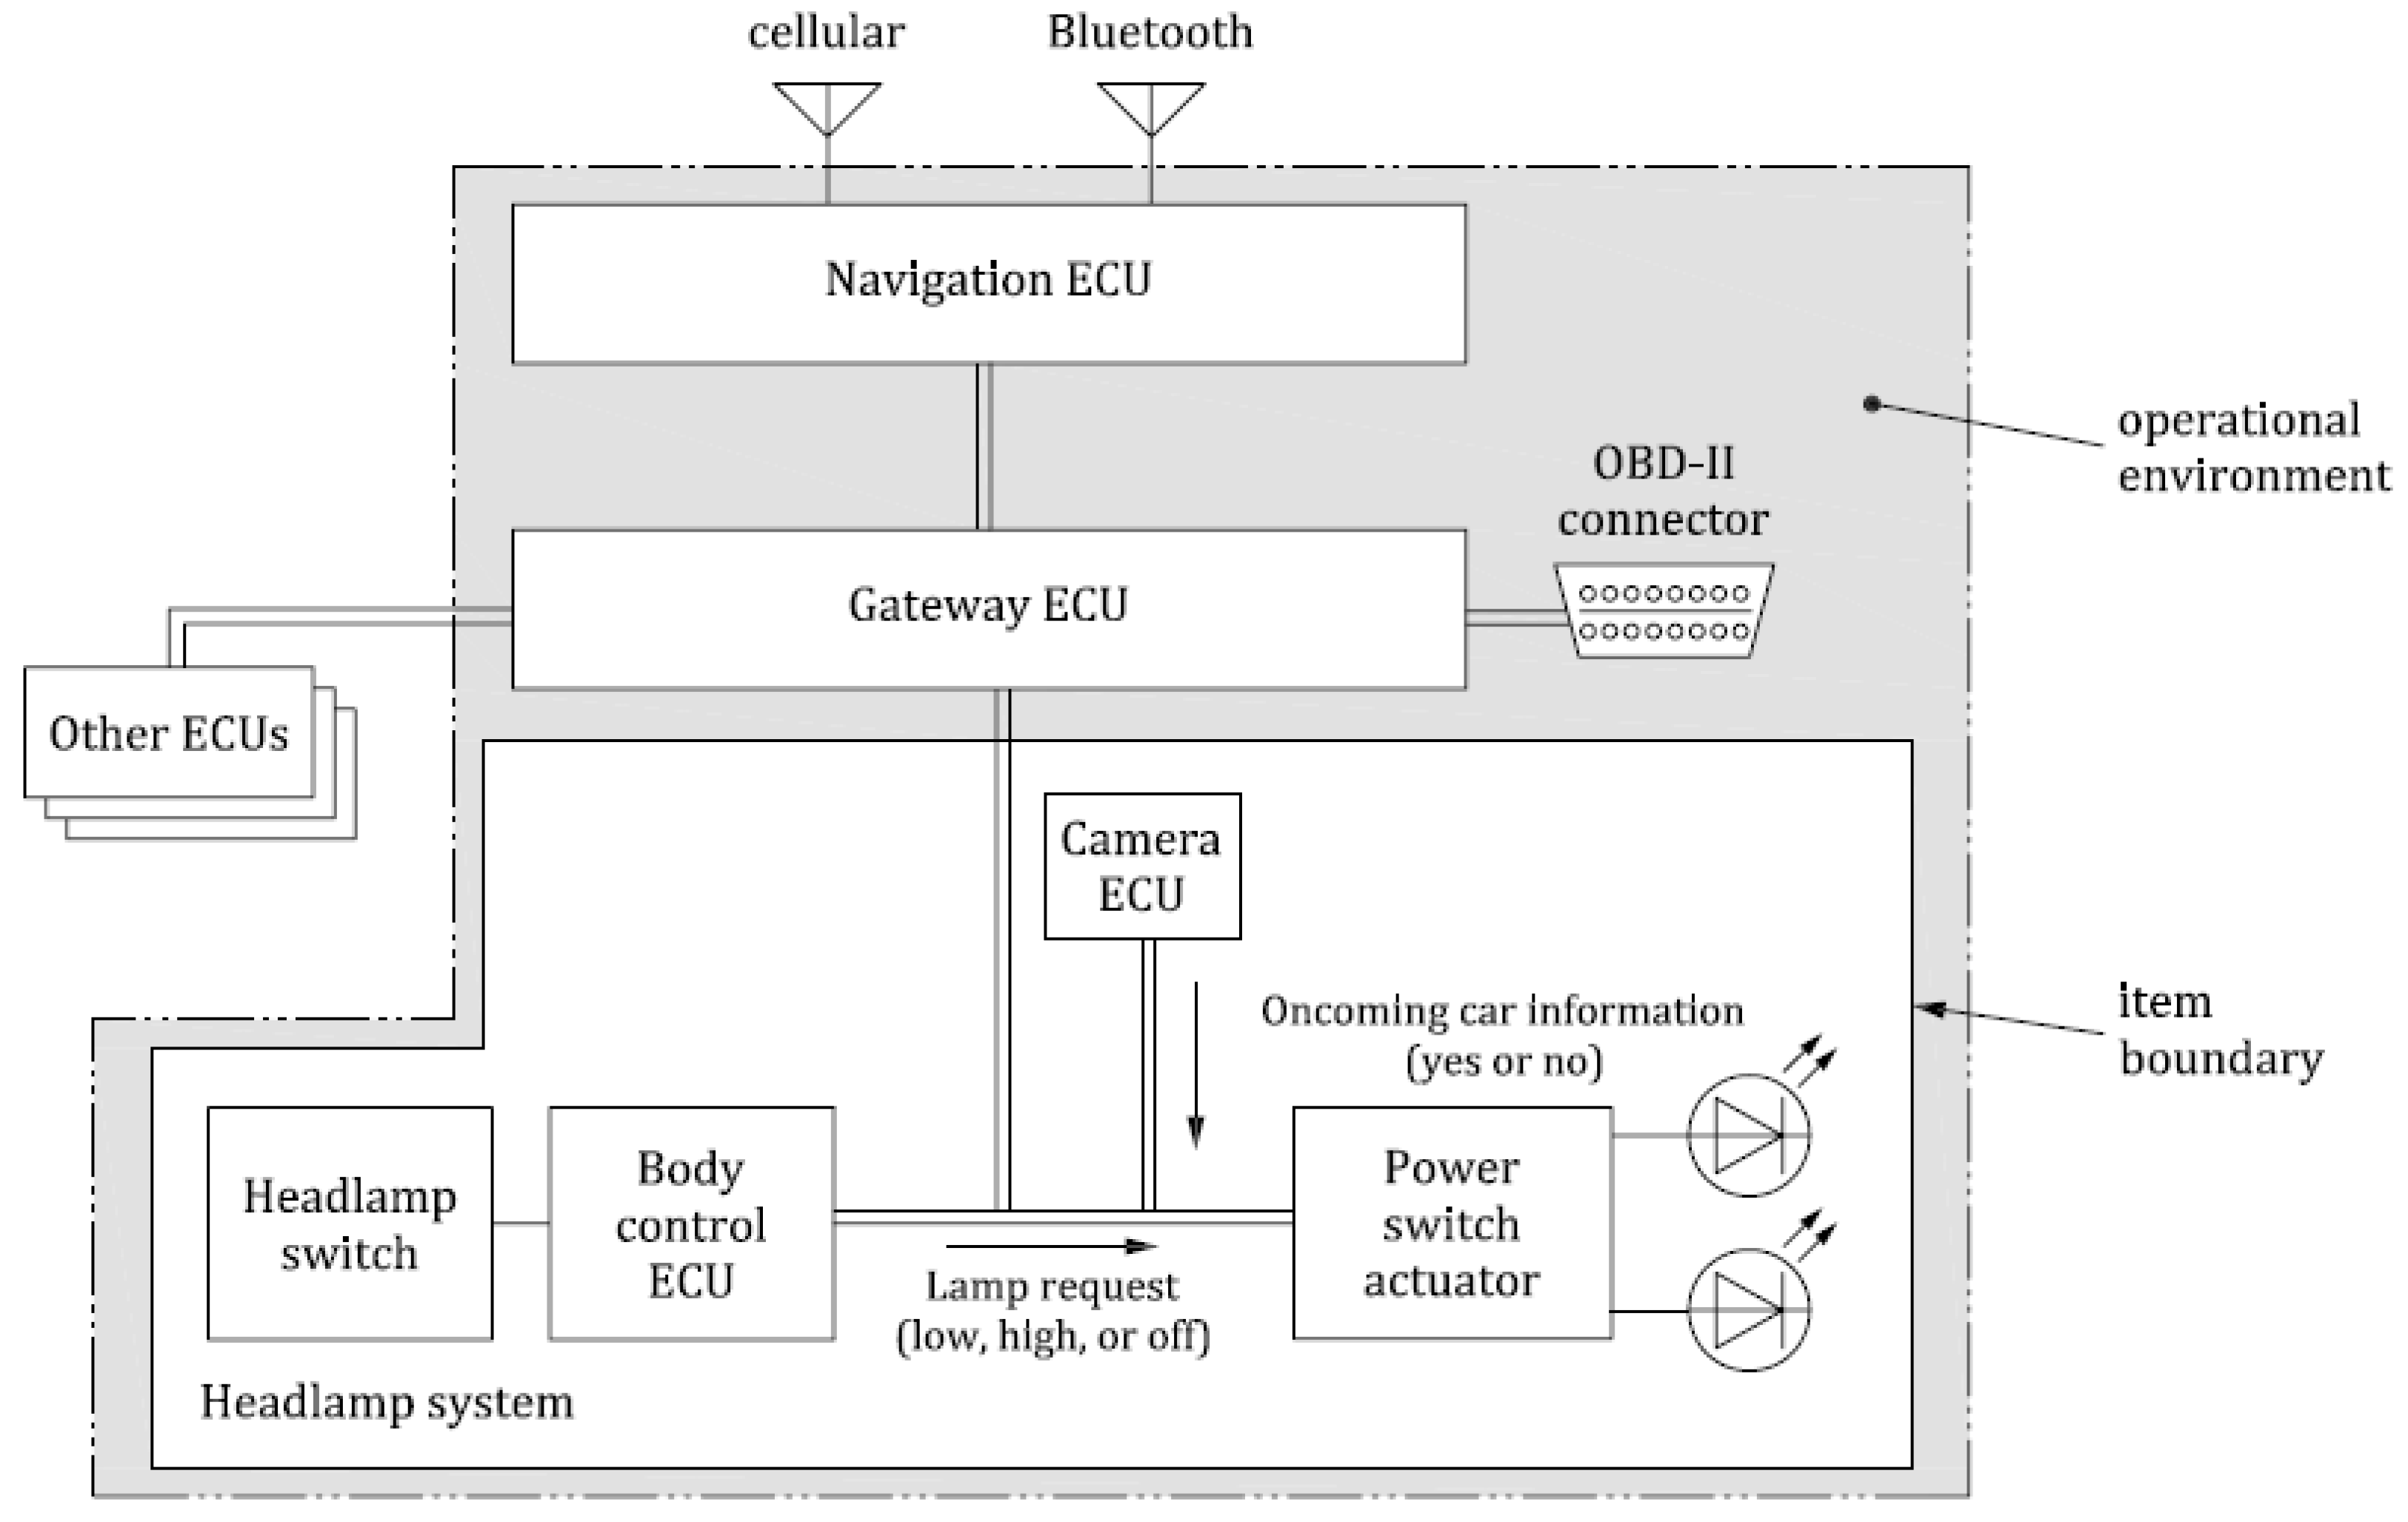
\includegraphics{s1.png}
        \vspace{-1em}
        \caption{Príklad \textbf{Itemu} analyzovaného v rámci TARA}
    \end{figure}
    \begin{itemize}
        \item \textbf{Item} = nejaký komponent systému, ktorý sa bude skúmať, na ktorom sa bude robiť TARA.
        \item Definícia jeho funkcii, aké má hranice, vzťah k ostatným častiam systému.
        \item TARA sa robí na každý item v systéme, ktorý je relevantný z hľadiska kybernetickej bezpečnosti.
        \item Definícia itemu nie je časť samotnej TARA, ale TARA sa vykonáva na definovaných itemoch.
    \end{itemize}
    \item Definícia \uv{\textbf{Asset}}-ov
    \begin{itemize}
        \item \textbf{Asset} je niečo, čo má hodnotu, čo musí byť chránené.
        \item CIA
    \end{itemize}
    \item Určenie \uv{\textbf{Damage scenarios}}
    \begin{itemize}
        \item Čo sa môže stať, ak by bol stratený asset? Aké sú \textbf{dôsledky} - čo zlé sa môže stať?
        \item Napríklad, ak by sa pokazila parkovacia kamera, tak damage scenario by mohlo byť že vodič pri parkovaní narazí do auta za ním, alebo že musí použiť spätné zrkadlo.
        \item Každé damage scenario má priradený \uv{impact} - napr. to, že na cúvanie sa musí použiť spätné zrkadlo, má menší impact ako niečo čo spôsobí čelnú kolíziu.
        \item Sú 4 typy damage scenarios: \uv{safety}, \uv{financial}, \uv{personal}, \uv{operational}
    \end{itemize}
    \item Určenie \uv{\textbf{Threat scenarios}}
    \begin{itemize}
        \item Čo môže spôsobiť damage scenario? 
        \item Napr. čo sa môže stať, aby to vyústilo v to, že sa pokazí parkovacia kamera -- môže sa pokaziť senzor, niekto sa na kameru mohol napojiť, atď.
        \item Opísané na vysokej úrovni, bez bližších detailov.
    \end{itemize}
    \item Určenie \uv{\textbf{Attack paths}}
    \begin{itemize}
        \item Ako zrealizovať threat scenario?
        \item Napr. ako by sa útočník vedel napojiť na kameru -- detailný opis krok za krokom.
        \item Pre jedno threat scenario môže existovať viac attack paths.
        \item Každý attack path má \textbf{feasibility rating} - ako ťažké je vykonať daný útok (napr. ak na vykonanie útoku musí útočník byť fyzicky v aute, znižuje to jeho feasibility rating).
    \end{itemize}
    \begin{figure}[H]
        \centering
        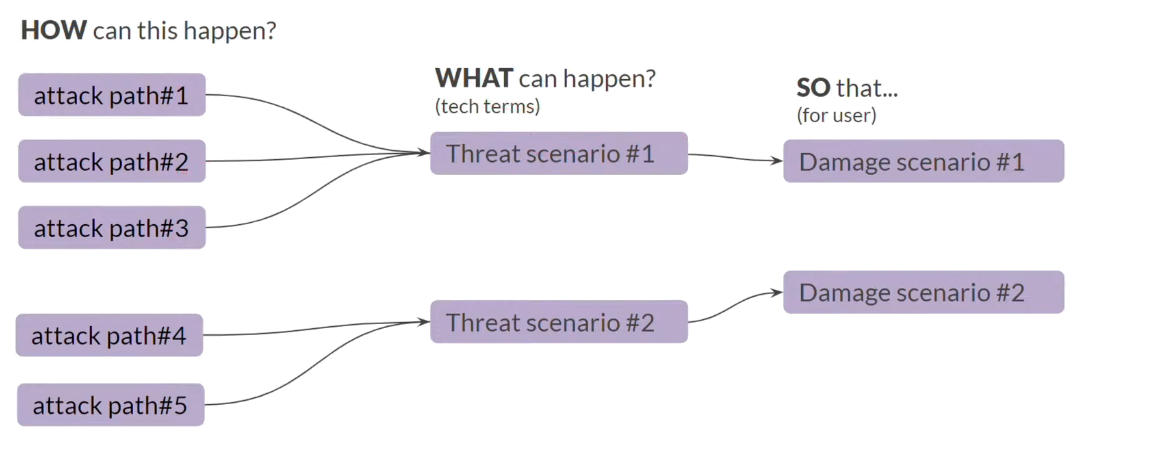
\includegraphics[width=\textwidth]{s2.png}
        \vspace{-2em}
        \caption{Vzťahy medzi \textbf{attack paths}, \textbf{threat scenarios} a \textbf{damage scenarios}}
    \end{figure}
    \item Kombináciou \textbf{impact ratingu} a korešpondujúceho \textbf{feasibility ratingu} sa vypočíta \textbf{risk value} - číslo medzi 1 a 5.
    \begin{figure}[H]
        \centering
        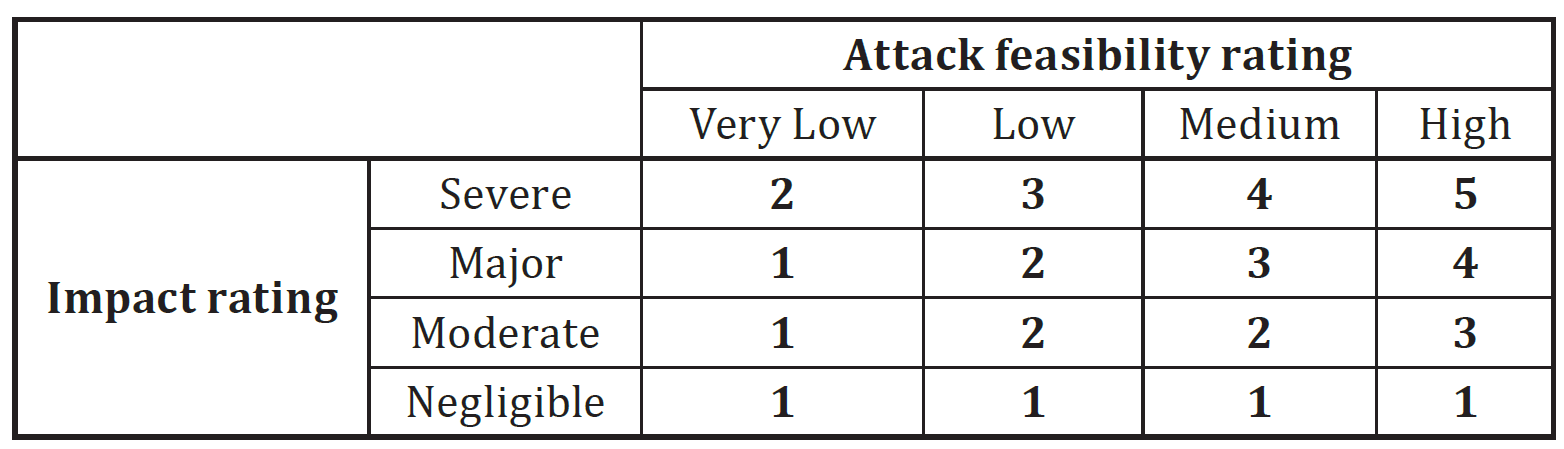
\includegraphics[width=\textwidth]{s3.png}
        \vspace{-2em}
        \caption{Príklad tabuľky pre určenie \textbf{risk value}}
    \end{figure}
    \item Vytvorenie \uv{\textbf{risk treatment options}} -- ako sa dá risk eliminovať (cybersecurity goals), alebo rozhodnutie, že je risk akceptovateľný, a mal by ponechať (cybersecurity claims).
\end{enumerate}

Kroky 3, 4, 5 sa môžu robiť v ľubovolnom poradí, t.j. môžme začať otázkou \uv{Čo sa môže stať?} (threat scenario), z toho určiť, aké to má následky (damage scenarios), a ako sa to môže stať (attack paths). V praxi sa to nerobí krok za krokom, ale jednotlivé kroky TARA analýzy sa vykonávajú v poradí, ktoré je pre daný prípad najvhodnejšie. Poradie samotné teda nie je dôležité, záleží iba na vzťahoch medzi jednotlivými threat scenarios, damage scenarios a attack paths navzájom.
    
\section{Databázy}

\subsection{MITRE ATT\&CK}

MITRE \textbf{ATT\&CK (Adversarial Tactics, Techniques, and Common Knowledge)} je databáza, ktorá katalogizuje reálne pozorované taktiky, techniky a postupy (TTP) používané útočníkmi pri kybernetických útokoch. Je postavená na reálnych dátach zo zaznamenaných bezpečnostných incidentov a slúži na pochopenie toho, ako útočníci v praxi postupujú v jednotlivých fázach útoku.

ATT\&CK je organizovaný do viacerých \textbf{matíc} (napr. Enterprise, Mobile, ICS), ktoré popisujú správanie útočníkov v rôznych prostrediach.

\begin{description}
    \item[ATT\&CK Enterprise] sa zameriava sa na tradičné business IT prostredie -- počítače, servery, cloud, identity, siete. Obsahuje techniky, ktoré útočníci používajú pri útoku na firemné informačné systémov (phishing, privilege escalation, exfiltrácia dát, atď.).

    \item[ATT\&CK Mobile] sa zameriava na útoky na mobilné zariadenia (Android, iOS). Matica zahŕňa techniky neautorizovaného prístupu k zariadeniam, vrátane tých, ktoré nevyžadujú fyzický prístup k zariadeniu.

    \item[ATT\&CK ICS (Industrial Control Systems)] je zameraný na riadenie priemyselných procesov -- bezpečnostné kontroléry, priemyselné protokoly, atď. Techniky obsajujú napriklad útoky na fyzické procesy, manipuláciu signálov, narušenie prevádzky alebo bezpečnostných mechanizmov. Je veľmi blízka oblasti embedded systémov a kritickej infraštruktúry.
\end{description}

\begin{itemize}
    \item Mapuje techniky (typy nápadov) na taktiky (ciele nápadov). Technika môže patriť do niekoľkých taktík.
    \item Dostupné verzie pre enterprise systémy, mobily a ICS. Pre autá je najviac použiteľná mobilná matica, prípadne matica ICS.
    \item Obranné opatrenia proti technikám: mitigations, detections, assets (nie je dostupné pre mobily).
\end{itemize}

Databáza ATT\&CK je dostupná vo formáte STIX dokumentu (podobný ako JSON). Jej najaktuálnejšiu podobu je možné získať aj pomocou API.

Myslíme, že pre náš projekt by bolo vhodné načítať a analyzovať tento STIX súbor, a následne ne jeho základne pripraviť dáta vo vlastnom formáte, ktorý je vhodnejší pre náš konkrétny prístup.

Vytvorili sme experimentálny TS skript, ktorý vie tento dokument načítať a spracovať. Na jeho základe sme zistili, že typy objektov, ktoré dokument obsahuje, a ktoré sú použiteľné pre náš projekt, sú \uv{\textbf{attack-pattern}}, \uv{\textbf{course-of-action}}, \uv{\textbf{x-mitre-detection-strategy}}, \uv{\textbf{tool}} (prípadne), a \uv{\textbf{relationship}}.

Okrem toho sme na základe JSON schémy STIX formátu vytovili sériu TypeScriptových typov, ktoré umožnia jednoduchšie využívanie a spracovanie takýchto dát.

\subsection{MITRE CAPEC}
MITRE \textbf{CAPEC (Common Attack Pattern Enumeration and Classification)} je verejne dostupná databáza známych \textbf{attack patterns} (vzorov útokov), ktorá slúži ako dokumentácia toho, ako útočníci typicky postupujú pri zneužívaní zraniteľností. CAPEC klasifikuje a popisuje jednotlivé útoky formou \uv{\textbf{attack patterns}} -- každý obsahuje informácie o mechanizme útoku, predpokladoch, možných dopadoch, potenciálnych mitigáciách a súvisiacich zraniteľnostiach.

Hoci CAPEC aj ATT\&CK sú oba projekty spravované MITRE, oba dokumentujú útoky na rôznych úrovniach detailu:
\begin{description}
    \item[CAPEC] opisuje vysoko abstraktné vzory útokov, teda čo útočník robí, aký je samotný \emph{princíp} útoku.
    \item[ATT\&CK] popisuje konkrétne taktiky, techniky a postupy (TTP) reálnych útočníkov v rôznych fázach útoku, teda ako reálne tieto útoky prebiehajú v praxi.
\end{description}

Medzi oboma systémami však existujú prepojenia -- mnohé ATT\&CK techniky odkazujú na príslušné CAPEC vzory, na ktorých sú založené. CAPEC je teda vhodný na pochopenie širšej logiky a princípov útokov, zatiaľ čo ATT\&CK je orientovaný na konkrétne scenáre používané v reálnom svete.

\subsection{MITRE CWE}

\textbf{CWE} sa hlavne zaoberá implementačnými/návrhovými slabinami softvéru, ktoré je potom možné využiť na napadnutie softvéru.

Databáza CWE ma tvar hierarchického stromu, prvkami ktorého sú uzly. Každý uzol definuje nejakú možnú zraniteľnosť systému a obsahuje meno, popis, cast zivotneho cyklusa systemu v ktorom sa objavi, potenciálne riešenia, výsledky, platne platformy a odkazy na vzory utokov z CAPEC ktore pouzivaju tu slabinu.

V závisloti od hĺbky, každý uzol môže mat typ \uv{Pillar}, \uv{Class}, \uv{Base}, alebo \uv{Variant}. Väčšina konkrétnych zraniteľností sú Base alebo Variant.

CWE taktiež poskytuje \uv{View} (pohľad), čo je skupina zraniteľností v závislosti od domény. Napríklad, poskytuje \uv{View} pre zraniteľnosti v softvére a zraniteľnosti v hardvéri.

\section{Návrh}
\subsection{Design}
\begin{figure}[H]
    \centering
    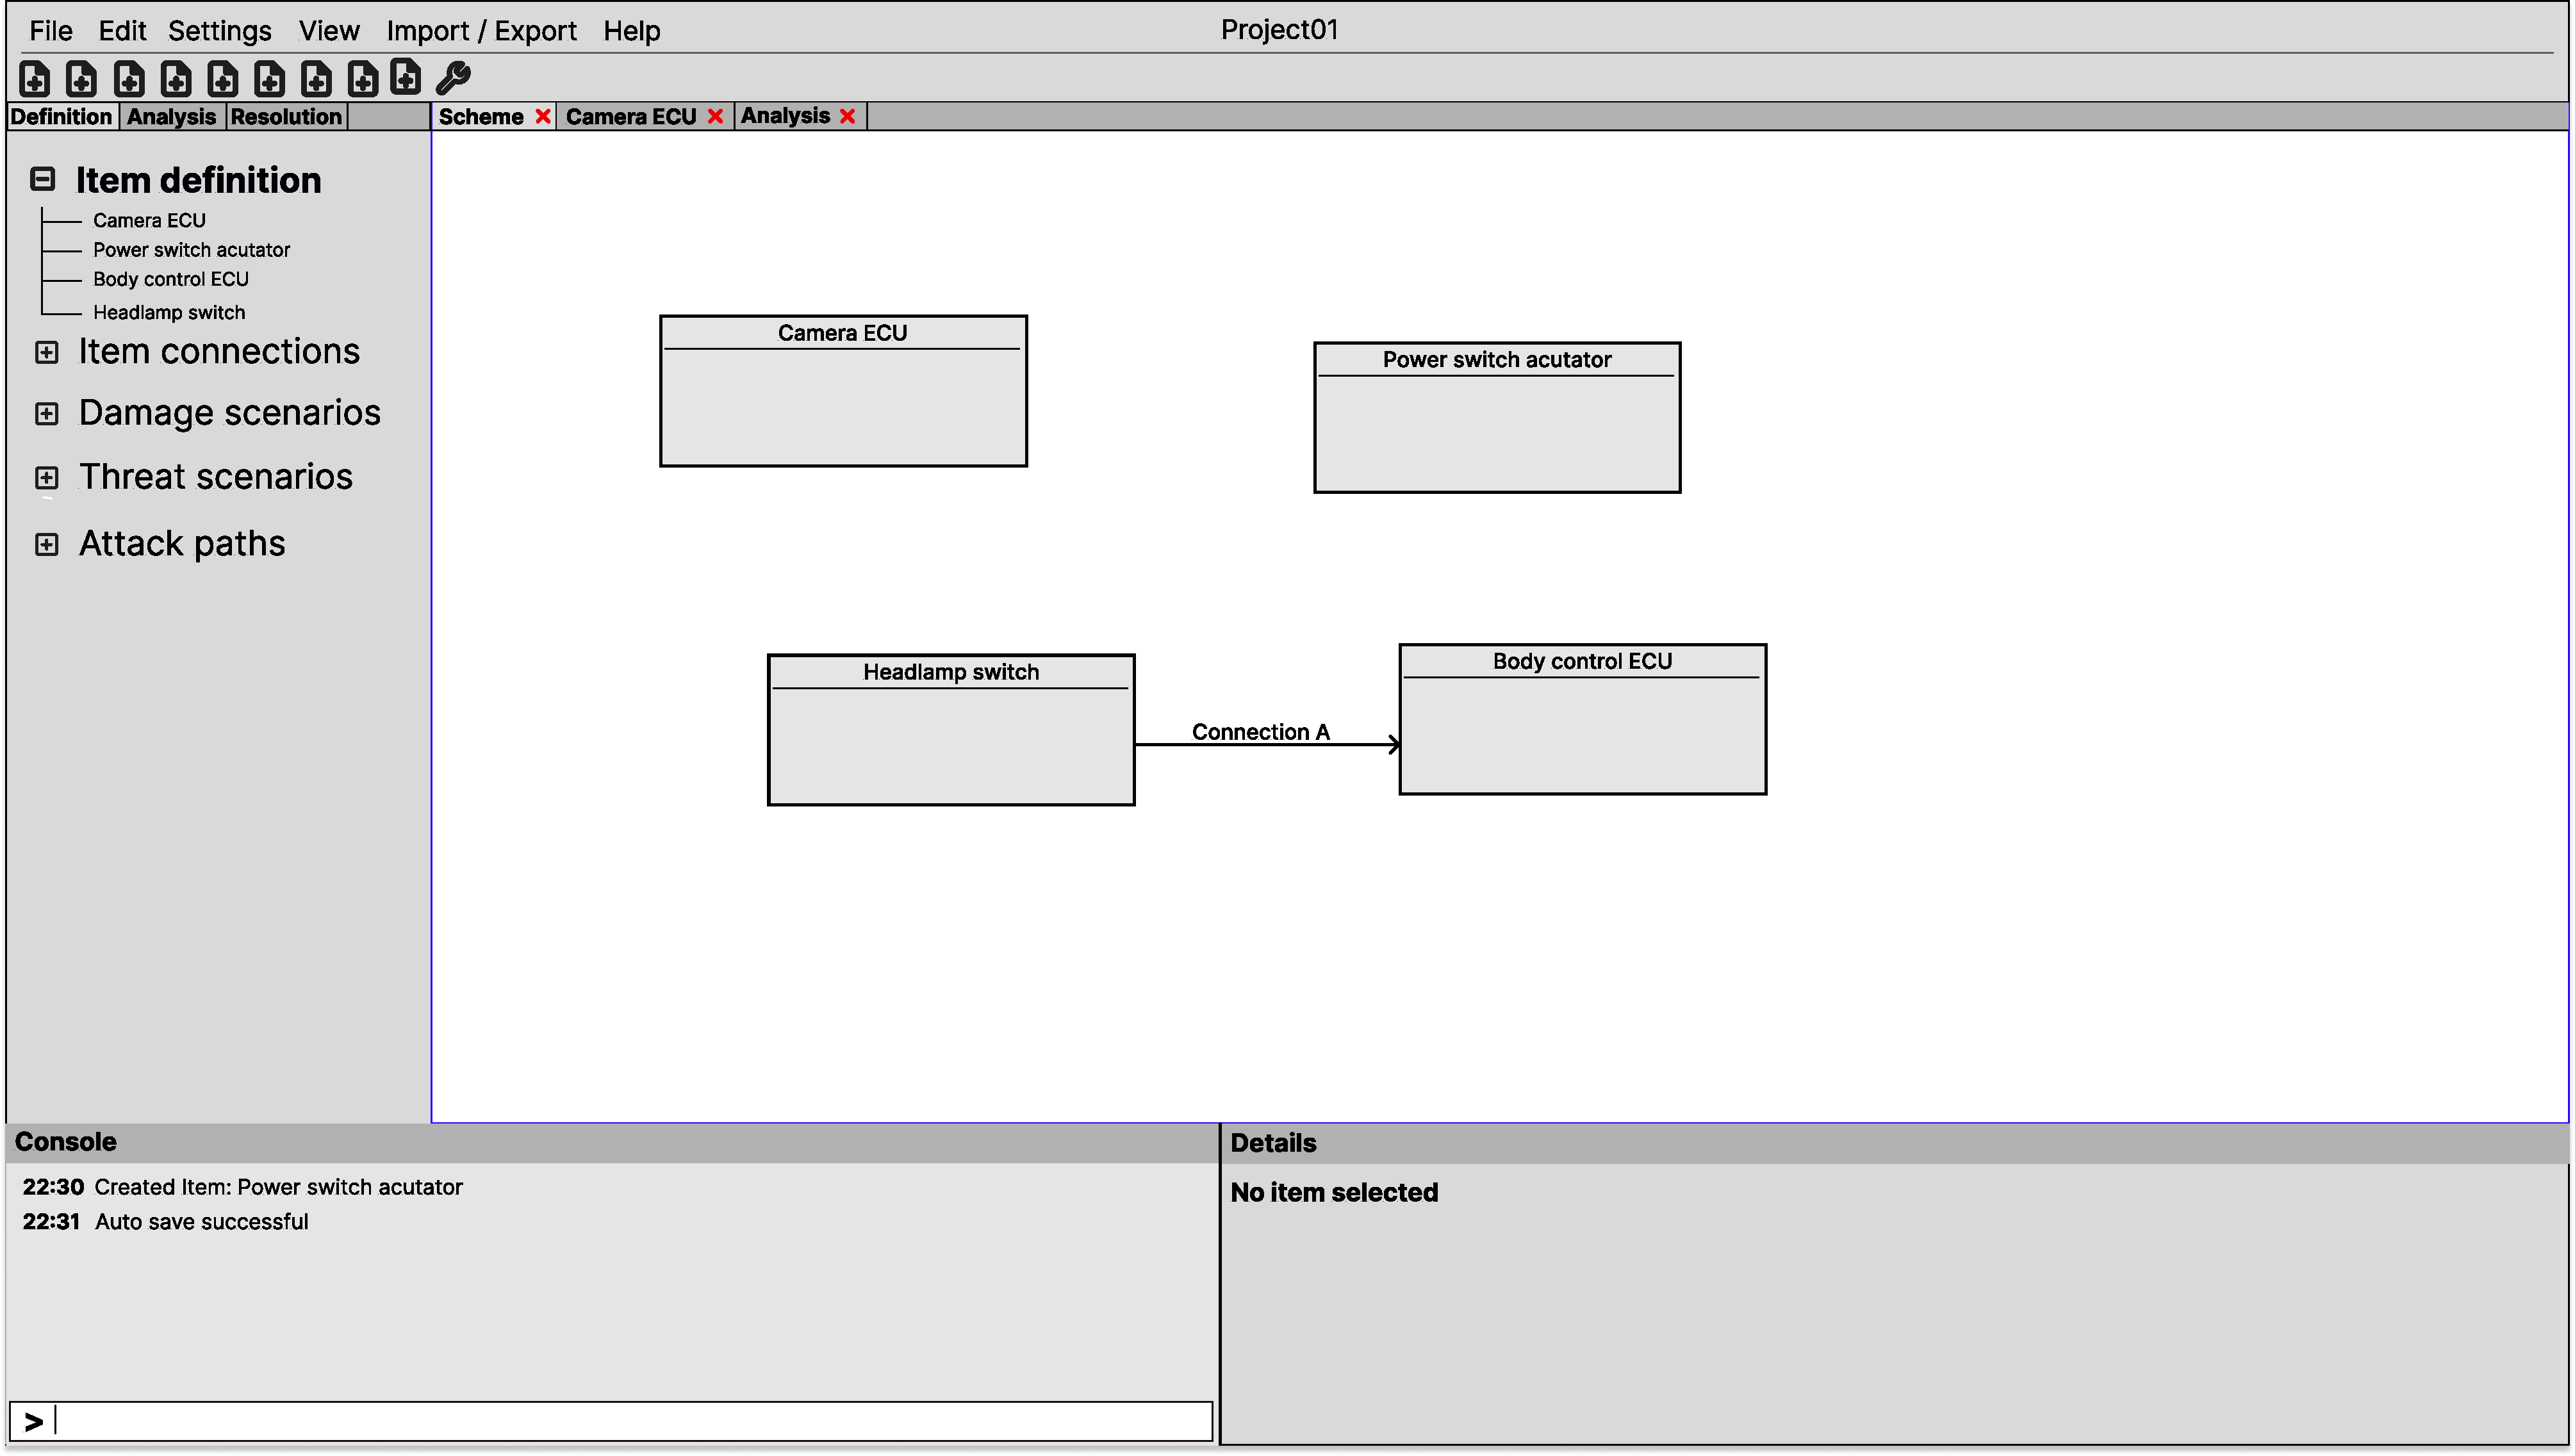
\includegraphics[width=\textwidth]{figma1.pdf}
    \caption{Prvý návrh aplikácie v nástroji figma}
    \label{figma1}
\end{figure}
Okno aplikácie sa skladá zo 6 základných častí:
\begin{enumerate}
    \item Navigácia - klasická všeobecne zaužívaná navigácia v hornej časti okna - obsahuje všetky základné aj pokročilé funkcie na správu projektov, nastavení a nastavenie aplikácie samotnej.
    \item Riadok s nástrojmi - určené pre nástroje používané pri práci s rôznymi časťami aplikácie. Tieto nástroje sa môžu meniť v závislosti od aktuálne otvoreného okna.
    \item Navigácia v ľavej časti obrazovky - Obsahuje položky \textbf{Definition} na definíciu samotného projektu. Tu sa vytvárajú itemy, damage scenarios, threat scenarios, attack paths a prepojenia medzi nimi. \textbf{Analysis} pre vyhodnotenie rizík. \textbf{Resolution} pre návrhy riešenia a rôzne iné poznámky.
    \item Hlavná časť aplikácie - obsahuje karty, ktoré sa otvárajú kliknutím na navigáciu v ľavej časti obrazovky alebo kliknutím na odkazy v hlavnej Časti aplikácie. Obsah kariet je už samotné jadro aplikácie - t.j. napríklad samotné vytváranie itemov prípadne spojení medzi nimi, vytváranie damage scenarios, výsledky analýzy a podobne.
    \item Console - Umožňuje uživateľovi zadávať príkazy, a zobrazuje históriu vykonaných akcii.
    \item Details - Zobrazuje detaily prvku ktorý je práve zakliknutý. Napríklad pri analýze môže uživateľ kliknúť na damage scenario, a v detailoch by sa mu o ňom zobrazili bližšie informácie. Ak by chcel uživateľ všetky informácie k danému prvku alebo by ho chcel modifikovať, mal by mať možnosť prvok jednoducho otvoriť aj ako okno v hlavnej časti aplikácie
\end{enumerate}
\subsection{Definovanie systému}
Na analýzu systému je najskôr potrebné definovať jeho časti, data ktoré používajú a vzťahy medzi nimi.
Na toto bude možné využiť systémový diagram alebo jednotlivé tabs pre konkrétne položky (komponenty, datové entity).
\subsubsection{Komponenty}
Základom všetkého budú komponenty, z ktorých budeme skladať analyzovaný systém.
Každý komponent bude mať svoje jedinečné ID, jeho názov a prípadný popis.
Tiež môže obsahovať \textbf{datové entity} a využívané \textbf{technológie}.

Pre komponenty budú definované vzťahy parent-child, pomocou ktorých bude možno jednoduchšie modelovať a agregovať hrozby na komponentoch.
Ďalším vzťahom bude vzťah komunikácie medzi komponentnmi, kde jeden komponent môže komunikovať s ďalším(i), pri tomto vzťahu je možné pre každý jednotlivý vzťah zadefinovať jeho názov.

Prvým/základným komponentom bude tzv. systémový komponent, ktorý bude obsahovať všetky komponenty projektu ako children.
\subsubsection{Datové entity}
Datové entity slúžia na reprezentáciu dát, ktoré používajú komponenty.
Každá datová entita bude mať svoje jedinečné ID, názov a prípadný popis dát ktoré reprezentuje.
\subsubsection{Technológie}
Technológie budú reprezentovať konkrétne technológie využívané v automobilovom priemysle (TCP/IP, UDP/IP, CAN bus, atď.).
Sú definované jedinečným ID, názvom a krátkym popisom.
Súčasťou aplikácie bude aj preddefinovaný list týchto technológií, ale uživateľ bude mať možnosť definovať vlastné, ak je to potrebné.
\begin{center}
    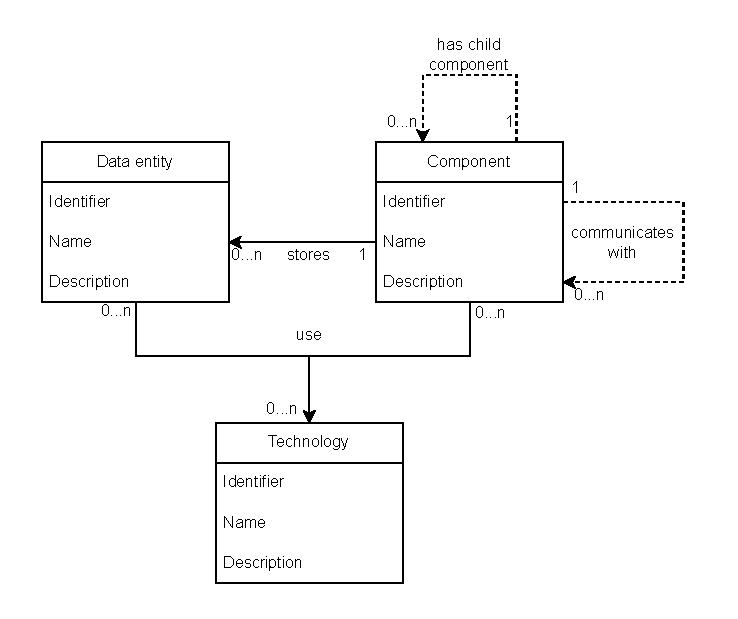
\includegraphics[width=0.75\textwidth]{erd-system.pdf}
\end{center}
\subsection{Identifikácia rizík}
Ďalšou súčasťou analýzy systému bude proces analýzy rizík, ktorý bude zjednodušený s využitím asistentov ktorý pomôžu vytvoriť scenáre poškodenia a korešpondujúce scenáre útoku pre jednotlivé datové entity alebo komponenty
\subsubsection{Asistent scenárov poškodenia}
Asistent scenárov poškodenia bude založený na dvoch krokoch, v prvom kroku uživatel prejde všetky komponenty/datové entity a určí, kde bude možné dôjsť k prípadnej hrozbe a označí, ktorú časť alebo časti CIA to ovplyvňuje.

Po prejdení všetkých komponentov a datových entít a určení hrozieb sa automaticky vytvoria kostry scenárov poškodenia pre všetky označené komponenty.
Uživatel ich následne môže upraviť, napríklad upraviť aká čast CIA je postihnutá týmto konkrétnym scenárom poškodenia.
Tiež môže doplniť položky impact scale, ktorý určuje počet zariadení ktoré môžu byť zasiahnuté a položku impact, ktorá definuje vplyv scenára na safety, financial, operational a privacy aspekty.

\subsubsection{Asistent scenárov hrozieb}
Asistent scenárov hrozieb bude využívať list definovaných hrozieb (budú existovať default hrozby ale uživatel bude môcť dodefinovať vlastné) ktoré bude posudzovať na komponentoch/data entitách kde boli určené scenáre poškodenia.

Následne budú scenáre hrozieb automaticky priradené k scenárom poškodenia, čím bude mať uživateľ zľahčenú prácu.
Pre kompletnosť scenára hrozby je potrebné dodefinovať kroky útoku, pomocou ktorých je hrozba realizovaná.

\subsubsection{Asistent krokov útoku}
Asistent scenárov tiež využíva list definovaných hrozieb a uživateľom definované scenáre hrozieb.
Pre každý scenár hrozby je vytvorený krok útoku, ktorý obsahuje informácie o tom, akú hrozbu spôsobuje, na akom komponente/datovej entite sa nachádza.

Uživatel môže dodefinovať controls ktoré dokážu zmierniť hrozbu alebo jej predísť, prípadne prípravný attack step, ktorý musí byť vykonaný pre fungovanie tohto.
Ďalším krokom bude vyplniť feasibility tabuľku, aby bol správne určený dopad kroku útoku na systém.

\subsubsection{Controls}
Controls slúžia na definovanie prvkov/opatrení, ktoré dokážu zmeniť dopad krokov útoku.
Pri ich definícií je potrebné uviesť názov, komponent alebo datovú entitu na ktorú sa aplikujú, na aké scenáre hrozby a kroky útoku mitigujú/sa aplikujú.
Tiež je potrebné zadefinovať feasibility tabuľku, ktorá bude definovať feasibility hodnoty po aplikovaní control.

Podobne ako pri technológiach, bude existovať list preddefinovaných controls (napr. symetrické šifrovanie, asymetrické šifrovanie) ktoré bude uživatel môcť použiť.

\begin{center}
    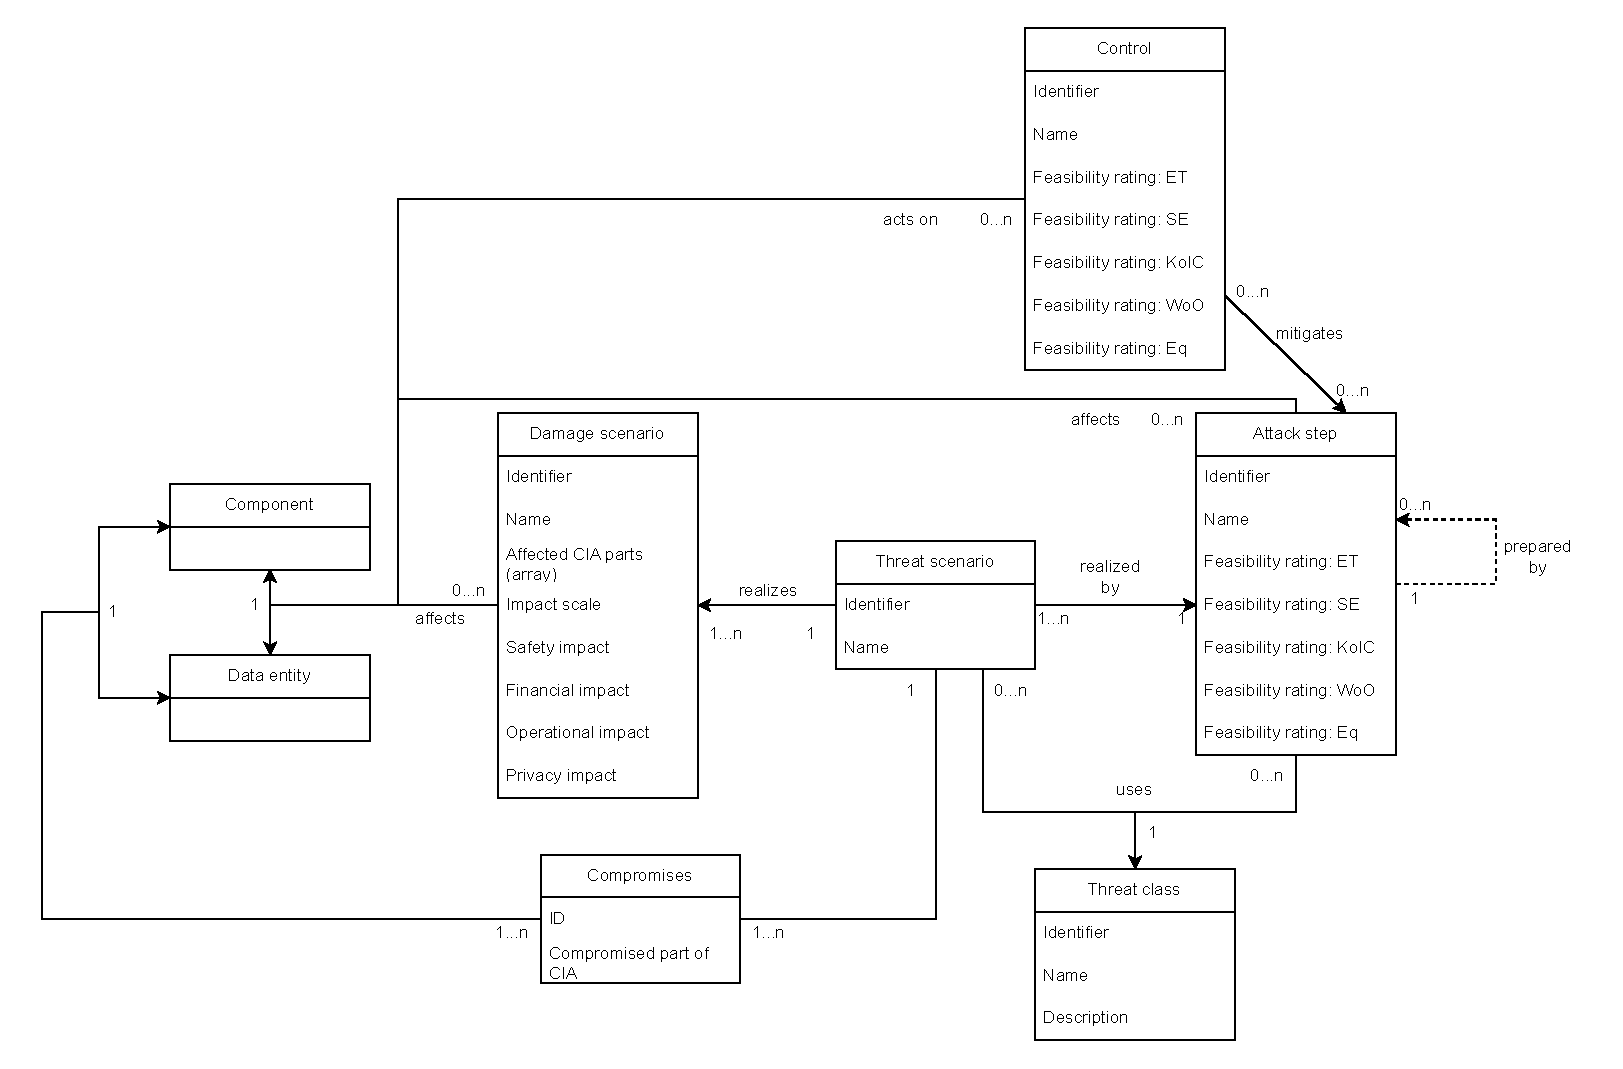
\includegraphics[width=0.85\textwidth]{erd-risks.pdf}
\end{center}

\subsection{Analýza rizík a mitigácia rizík}
Na analýzu rizík budú používané control skupiny definované používateľom, ktoré umožnia vytvárať rôzne kombinácie opatrení ktoré bude môcť porovnávať.

Výsledok analýzy je následne možné exportovať ako dokument, ktorý bude obsahovať informácie o systéme, scenároch poškodenia, hrozieb a aj krokoch útoku.
Tiež bude obsahovať control opatrenia a ako sú aplikované na jednotlivé kroky útoku/scenáre hrozieb, kde bude jasné vidieť ktoré z nich boli alebo neboli "opravené" opatreniami.

Ďalším nástrojom na analýzu a mitigáciu rizík bude možnosť použitia LLM, ktorý bude môcť využiť na analýzu alebo pomoc pri definovaní systému.

\subsubsection{Control skupiny}
Skupiny control opatrení budú definované uživatelom, s tým že budú existovať dve predvolené nastavenia, kde nebudú aplikované žiadne opatrenia, alebo naopak, kde sú aplikované všetky control opatrenia.

Uživatel bude môcť vytvoriť ďalšie skupiny, kde bude môcť definovať ich meno, prípadný popis a potom bude môcť priradiť jednotlivé control opatrenia.

\subsubsection{Využitie LLM}
Uživatel bude mať možnosť využit LLM (buď lokálny model, alebo vie nastaviť využitie modelu cez ich API) na prácu s definovaným systémom v aplikácií.

Prvou možnosťou bude využitie nástrojov (implementované pomocou LangChain Tools), ktorými bude možné vytvoriť komponenty/datové entity napísaním inštrukcii LLM (napr. "vytvor ECU komponent ktorý obsahuje 3 data entity a má podkomponent..."), čím sa značne zjednoduší proces modelovania systému.

Ďalšou možnosťou bude vykonávať analýzu nad vytvoreným systémom, kde bude mať model (ak to uživatel povolí) prístup ku kontextu systému a bude môcť analyzovať jeho časti podľa štandardu.

\subsection{Backend}
Backend server bude implementovaný použitím technológii \texttt{django} spolu s \texttt{rest framework} (\url{https://www.django-rest-framework.org/}). Okrem manipulácie s databázou bude server zabezpečovať autorizáciu a vnútornú logiku aplikácie. Nižšie sú popísané endpointy backend servera slúžiace na komunikáciu s frontendom. Na týchto endpointoch bude server príjmať alebo posielať JSON dáta.  Pri každom z nižšie uvedených endpointov je aj príklad dát, ktoré server očakáva (pre POST požiadavky) alebo odosiela (pre GET požiadavky). Uvedené sú iba názvy JSON polí, ich hodnoty sú vynechané. \\

\textbf{GET /api/component}
\begin{verbatim}
{component: [
    {id, name, description},
    {id, name, description}
]}
\end{verbatim}

\vspace{1cm}
\textbf{POST /api/component}
\begin{verbatim}
{name, description, data_entities: [data_entity_id1, data_entity_id2], 
technologies: [technology_id1, technology_id2]}
\end{verbatim}

\vspace{1cm}
\textbf{GET /api/component/$<$id$>$}
\begin{verbatim}
{id, name, description, data_entity: [
        {id, name, description},
        {id, name, description},
    ], 
	technology: [
		{id, name, description},
		{id, name, description}
	],
	damage_scenario: [
		{id, name, affected_CIA_parts, impact_scale, safety_impact, finantial_impact, 
        operational_impact, privacy_impact, threat_scenario_id},
		{id, name, affected_CIA_parts, impact_scale, safety_impact, finantial_impact, 
        operational_impact, privacy_impact, threat_scenario_id}
	],
	control: [control_id1, control_id2],
	threat_scenarios: [threat_scenario_id1, threat_scenario_id2],
	attack_steps: [attack_step_id1, attack_step_id2],
	}
\end{verbatim}
\vspace{1cm}
\textbf{POST /api/component/$<$id$>$} 
\begin{verbatim}
{name, description, data_entity: [
        {id, name, description},
        {id, name, description},
    ], 
	technology: [
		{id, name, description},
		{id, name, description}
	],
	damage_scenario: [
		damage_scenario_id1, damage_scenario_id2
	],
	control: [control_id1, control_id2],
	threat_scenarios: [threat_scenario_id1, threat_scenario_id2],
	attack_steps: [attack_step_id1, attack_step_id2],
	}
\end{verbatim}

\vspace{1cm}
\textbf{GET /api/damage\_scenario} 
\begin{verbatim}
{damage_scenario : [
		{id, name, affected_CIA_parts, impact_scale, safety_impact, finantial_impact, 
        operational_impact, privacy_impact, threat_scenario_id, component_id}, 
		{id, name, affected_CIA_parts, impact_scale, safety_impact, finantial_impact, 
        operational_impact, privacy_impact, threat_scenario_id, component_id}
	]}
\end{verbatim}

\vspace{1cm}
\textbf{POST /api/damage\_scenario} 
\begin{verbatim}
{name, affected_CIA_parts, impact_scale, safety_impact, finantial_impact, 
operational_impact, privacy_impact, threat_scenario_id, component_id}
\end{verbatim}

\vspace{1cm}
\textbf{GET /api/damage\_scenario/component/$<$component\_id$>$}\\ 
(Rovnaké ako \texttt{GET /api/damage\_scenario}, ale vyfiltrované pre komponent s daným id)

\vspace{1cm}
\textbf{GET /api/damage\_scenario/$<$id$>$} 
\begin{verbatim}
{id, name, affected_CIA_parts, impact_scale, safety_impact, finantial_impact, 
operational_impact, privacy_impact, threat_scenario_id, component_id}
\end{verbatim}

\vspace{1cm}
\textbf{POST /api/damage\_scenario/$<$id$>$} 
\begin{verbatim}
{name, affected_CIA_parts, impact_scale, safety_impact, finantial_impact, 
operational_impact, privacy_impact, threat_scenario_id, component_id}
\end{verbatim}

\vspace{1cm}
\textbf{GET /api/control} 
\begin{verbatim}
control: [
    {id, name, fr_et, fr_se, fr_koC, fr_WoO, fr_eq, component_id, 
    attack_steps: [attack_step_id1, attack_step_id2]},
    {id, name, fr_et, fr_se, fr_koC, fr_WoO, fr_eq, component_id, 
    attack_steps: [attack_step_id1, attack_step_id2]},
]
\end{verbatim}

\vspace{1cm}
\textbf{POST /api/control} 
\begin{verbatim}
{name, fr_et, fr_se, fr_koC, fr_WoO, fr_eq, component_id, 
attack_steps: [attack_step_id1, attack_step_id2]}
\end{verbatim}

\vspace{1cm}
\textbf{GET /api/control/component/$<$component\_id$>$}\\ 
(Rovnaké ako \texttt{GET /api/control}, ale vyfiltrované pre komponent s daným id)

\vspace{1cm}
\textbf{GET /api/control/$<$id$>$} 
\begin{verbatim}
{id, name, fr_et, fr_se, fr_koC, fr_WoO, fr_eq, component_id, 
attack_steps: [attack_step_id1, attack_step_id2]}
\end{verbatim}

\vspace{1cm}
\textbf{POST /api/control/$<$id$>$} 
\begin{verbatim}
{name, fr_et, fr_se, fr_koC, fr_WoO, fr_eq, component_id, 
attack_steps: [attack_step_id1, attack_step_id2]}
\end{verbatim}

\vspace{1cm}
\textbf{GET /api/attack\_step} 
\begin{verbatim}
attack_step: [
	{id, name, fr_et, fr_se, fr_koC, fr_WoO, fr_eq, prepared_by: [
			{id, name, fr_et, fr_se, fr_koC, fr_WoO, fr_eq, prepared_by},
			{id, name, fr_et, fr_se, fr_koC, fr_WoO, fr_eq, prepared_by}
			], component_id, threat_class_id, threat_scenario: [
				threat_scenario_id1, threat_scenario_id2
			], controls: [
				controls_id_1, controls_id_2
			] },
	{id, name, fr_et, fr_se, fr_koC, fr_WoO, fr_eq, prepared_by: [
			{id, name, fr_et, fr_se, fr_koC, fr_WoO, fr_eq, prepared_by},
			{id, name, fr_et, fr_se, fr_koC, fr_WoO, fr_eq, prepared_by}
			], component_id, threat_class_id, threat_scenario: [
				threat_scenario_id1, threat_scenario_id2
			], controls: [
				controls_id_1, controls_id_2
			] },
]
\end{verbatim}

\vspace{1cm}
\textbf{POST /api/attack\_step} 
\begin{verbatim}
{id, name, fr_et, fr_se, fr_koC, fr_WoO, fr_eq, prepared_by: [
			attack_step_id1, attack_step_id2
			], component_id, threat_class_id, threat_scenario: [
				threat_scenario_id1, threat_scenario_id2
			], controls: [
				controls_id_1, controls_id_2
			] },
\end{verbatim}

\vspace{1cm}
\textbf{GET /api/attack\_step/component/$<$component\_id$>$}\\ 
(Rovnaké ako \texttt{GET /api/attack\_step}, ale vyfiltrované pre komponent s daným id)

\vspace{1cm}
\textbf{GET /api/attack\_step/$<$id$>$} 
\begin{verbatim}
{id, name, fr_et, fr_se, fr_koC, fr_WoO, fr_eq, prepared_by: [
	{id, name, fr_et, fr_se, fr_koC, fr_WoO, fr_eq, prepared_by},
	{id, name, fr_et, fr_se, fr_koC, fr_WoO, fr_eq, prepared_by}
	], component_id, threat_class_id, threat_scenario: [
		threat_scenario_id1, threat_scenario_id2
	], controls: [
		controls_id_1, controls_id_2
	] }
\end{verbatim}

\vspace{1cm}
\textbf{POST /api/attack\_step/$<$id$>$} 
\begin{verbatim}
{name, fr_et, fr_se, fr_koC, fr_WoO, fr_eq, prepared_by: [
	attack_step_id1, attack_step_id2
	], component_id, threat_class_id, threat_scenario: [
		threat_scenario_id1, threat_scenario_id2
	], controls: [
		controls_id_1, controls_id_2
	] }
\end{verbatim}

\vspace{1cm}
\textbf{GET /api/threat\_scenario} 
\begin{verbatim}
{ threat_scenario: [
	{id, name, attack_step: [attack_step_id1, attack_step_id2], 
    damage_scenario: [damage_scenario_id1, damage_scenario_id2], 
    threat_class_id, compromises: [
	{component_id, compromised_part_cia},
	{component_id, compromised_part_cia}]},
	{id, name, attack_step: [attack_step_id1, attack_step_id2], 
    damage_scenario: [damage_scenario_id1, damage_scenario_id2], 
    threat_class_id, compromises: [
	{component_id, compromised_part_cia},
	{component_id, compromised_part_cia}]},
	]}
\end{verbatim}

\vspace{1cm}
\textbf{POST /api/threat\_scenario} 
\begin{verbatim}
{name, attack_step: [attack_step_id1, attack_step_id2], 
damage_scenario: [damage_scenario_id1, damage_scenario_id2], 
threat_class_id, compromises: [
	{component_id, compromised_part_cia},
	{component_id, compromised_part_cia}]},
	]}
\end{verbatim}

\vspace{1cm}
\textbf{POST /api/threat\_scenario/component/$<$component\_id$>$}\\
(Rovnaké ako \texttt{GET /api/threat\_scenario}, ale vyfiltrované pre komponent s daným id)

\vspace{1cm}
\textbf{GET /api/threat\_scenario/$<$id$>$} 
\begin{verbatim}
{id, name, attack_step: [attack_step_id1, attack_step_id2], 
damage_scenario: [damage_scenario_id1, damage_scenario_id2], 
threat_class_id, compromises: [
	{component_id, compromised_part_cia},
	{component_id, compromised_part_cia}]}
\end{verbatim}

\vspace{1cm}
\textbf{POST /api/threat\_scenario/$<$id$>$} 
\begin{verbatim}
{name, attack_step: [attack_step_id1, attack_step_id2], 
damage_scenario: [damage_scenario_id1, damage_scenario_id2], 
threat_class_id, compromises: [
	{component_id, compromised_part_cia},
	{component_id, compromised_part_cia},
]}
\end{verbatim}

\vspace{2cm}
Jednoduchý prototyp backend servera je k dispozícii na \url{https://github.com/oldo7/TP_team12_backend}

\section{Frontend}
\subsection{Návrh a prototyp aplikácie}
Na vytvorenie frontendu vyvíjanej aplikácie sme sa rozhodli použiť technológiu React v kombinácii s nástrojom Vite ako vývojovým bundlerom. Technológie volíme prevažne kvôli tomu, že sú moderné, široko používané a poskytujú rýchle vývojové prostredie. React umožňuje rozdeľovanie GUI na menšie logické segmenty, čím sa výrazne uľahčuje vývoj.

Pri vývoji využívame doplnkové knižnice, napríklad hlavne shadcn, Tailwind a Lucide, pomocou ktorých vytvárame konzistentné, moderné a vizuálne zjednotené prostredie. Pri návrhu homepage sme sa inšpirovali dizajnom z nástroja Figma zobrazeného na \nameref{figma1}.

V aktuálnej fáze projektu bol vytvorený funkčný prototyp frontendovej časti aplikácie. Prototyp obsahuje základné rozloženie homepage, rozloženie hlavných komponentov a demonštračné dáta, ktoré slúžia ako zástupné hodnoty. Na obrázku nižšie je uvedený screenshot aktuálneho stavu prototypu aplikácie, ktorý zobrazuje základné rozhranie a štruktúru frontendovej časti. (\nameref{frontend_prototype})

\begin{figure}[H]
    \centering
    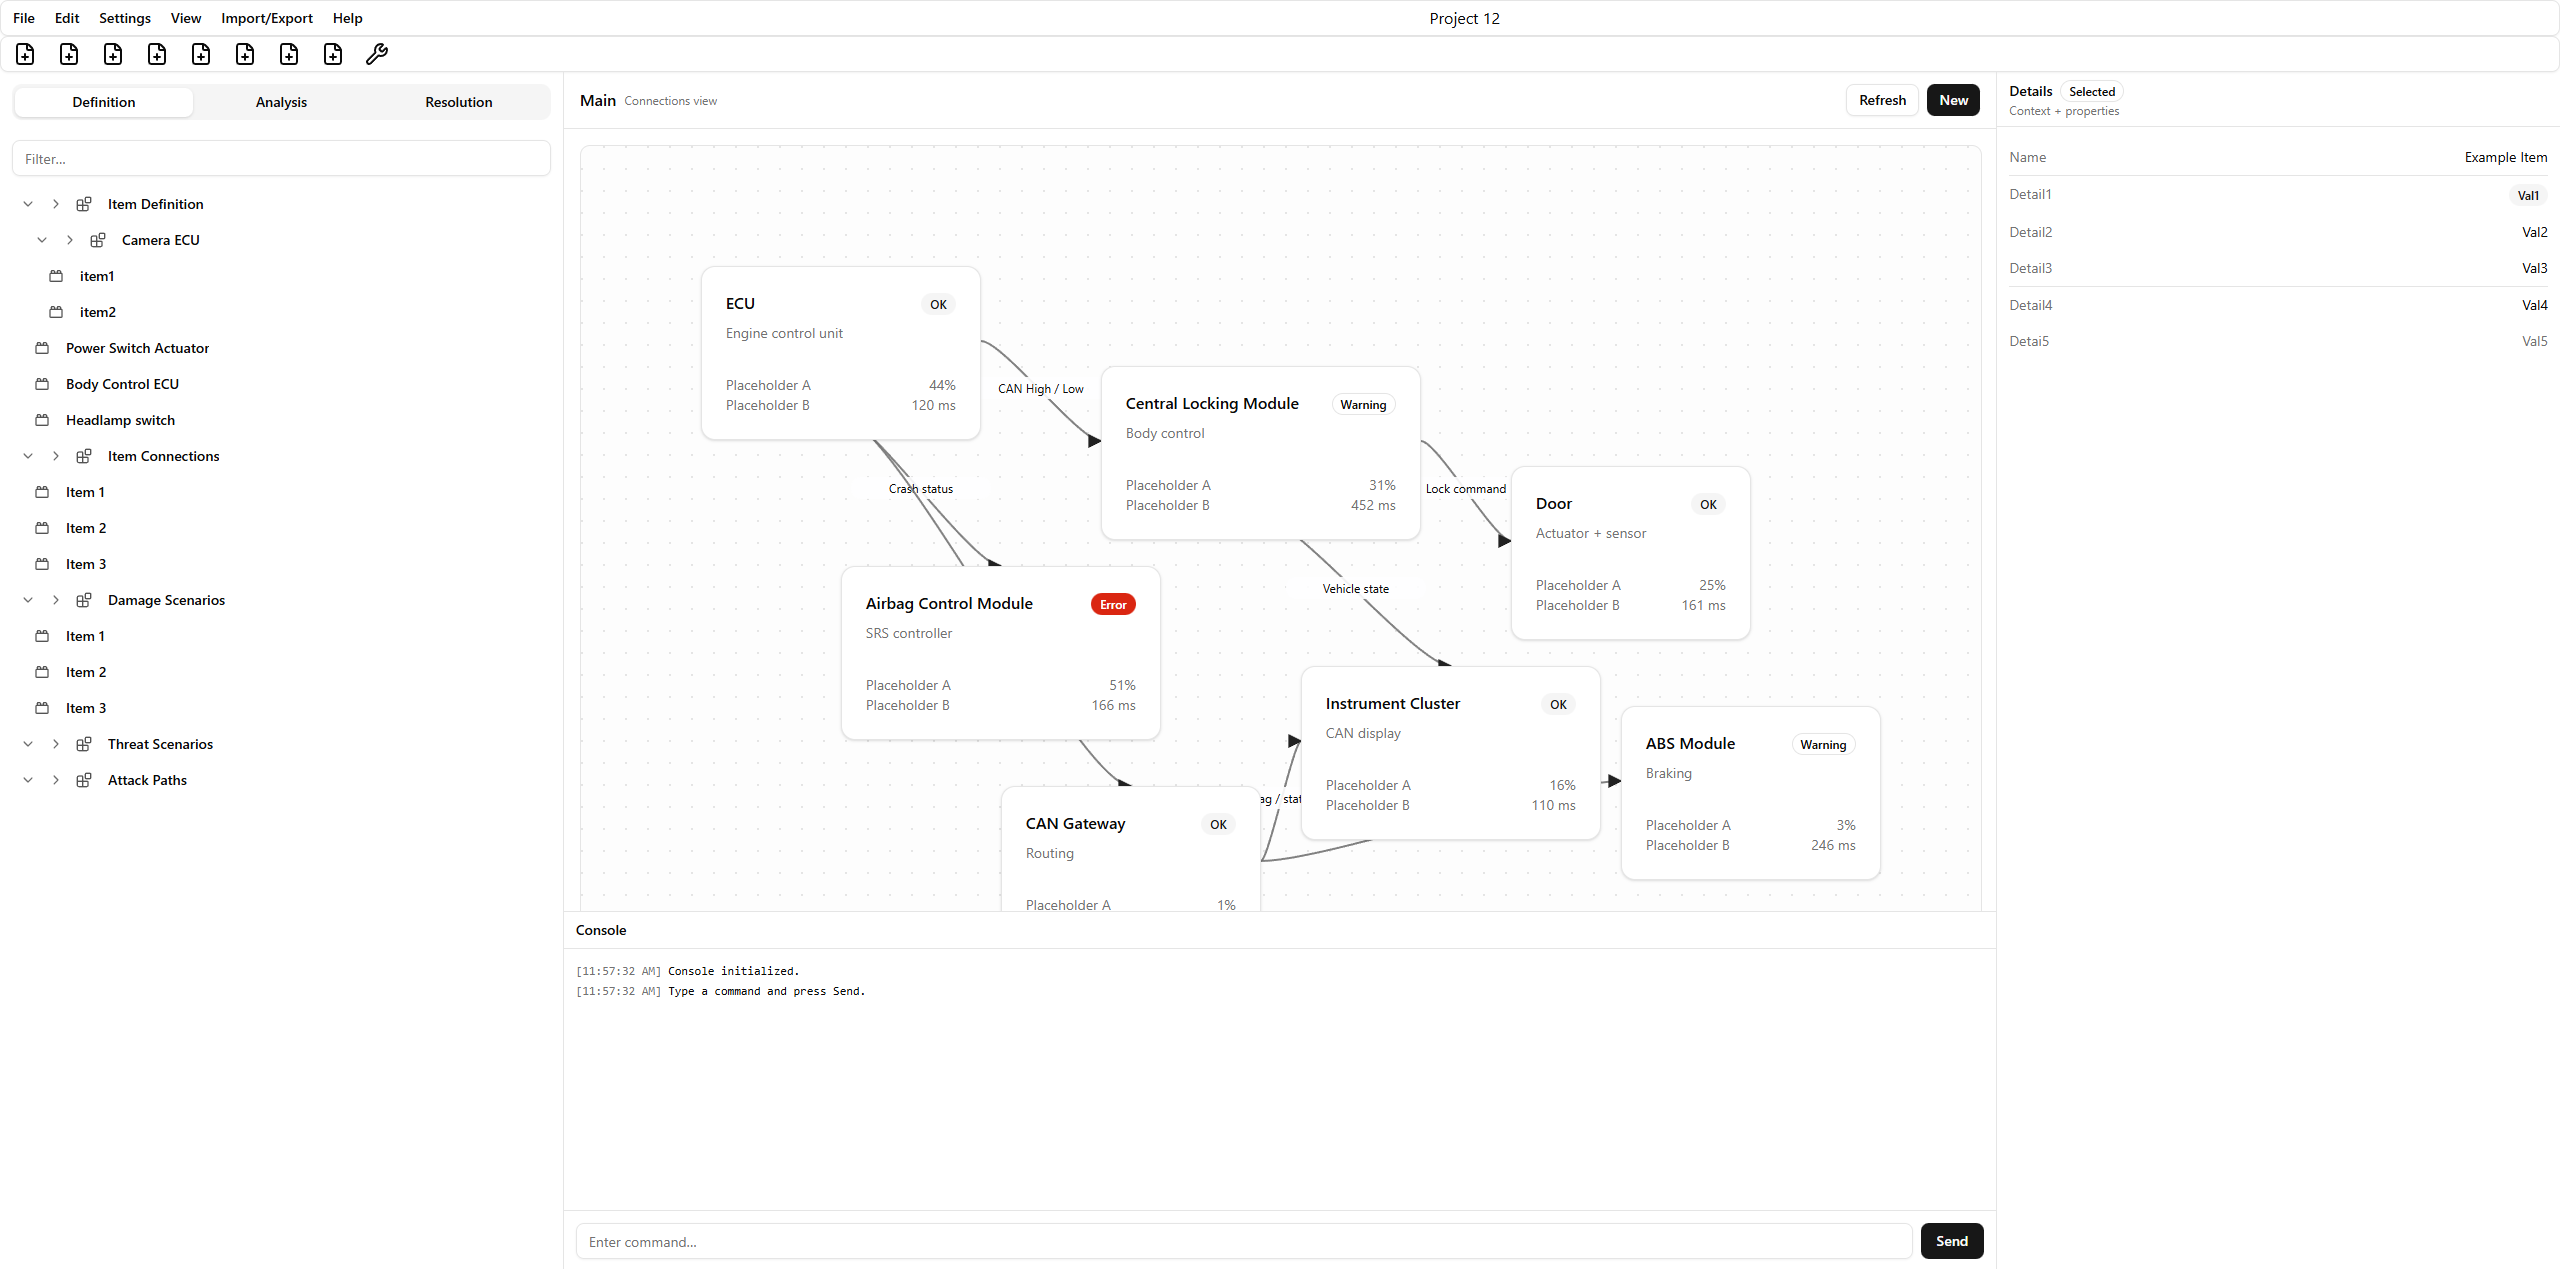
\includegraphics[width=\textwidth]{frontend_prototype.png}
    \caption{Prototyp Frontendovej časti}
    \label{frontend_prototype}
\end{figure}

Zdrojový kód základného návrhu projektu nájdete tu: \url{https://github.com/rykktiadloans/TP_team12_frontend} (Prípadne: \url{https://github.com/Fer1SK/TP_team12_frontend/tree/main})

\section{Backend - Iterácia 2}
V tejto iterácii boli dokončené všetky endpointy, boli pridané projekty a ostatné CRUD operácie pre všetky databázové objekty. Tiež bola pridaná autentizácia a autorizácia uživateľa pomocou JWT.

\subsection{Autentizáia a autorizácia}
Uživateľ bude mať možnosť si vytvoriť účet, a ku svojmu účtu bude mať následne priradené projekty. V rámci projektov potom už bude mať jednotlivé komponenty, damage scenaria a ostatné. V prvom kroku si uživateľ vytvorí účet pomocou nasledovného API callu:

\begin{verbatim}
POST /api/register/
Content-Type: application/json
{
  "username": "Oliver",
  "password": "heslo123",
  "email": "oliver@example.com"
}
\end{verbatim}
Ako odpoveď je z backendu odoslané potvrdenie o vytvorení uživateľa. Keď už uživateľ má účet, môže sa prihlásiť pomocou nasledovného API callu:
\begin{verbatim}
POST /api/token/
Content-Type: application/json
{
  "username": "john_doe",
  "password": "securepass123"
}
\end{verbatim}
Odpoveďou je JSON Web Token (poznámka: namiesto \verb|<|JWT\verb|>| bude v praxi base64 enkódovaný string):
\begin{verbatim}
{
  "access": <accessJWT>,
  "refresh": <refreshJWT>"
}
\end{verbatim}
Tento token následne uživateľ odosiela v každej požiadavke v hlavičke:
\begin{verbatim}
Authorization: Bearer <accessJWT>
\end{verbatim}
Na základe tohto tokenu sa overí, či má prístup ku projektu, ktorého sa požiadavka týka. V prípade že uživateľovi token vyprší, môže si ho obnoviť použitím nasledujúceho API callu:
\begin{verbatim}
POST /api/token/refresh/
Content-Type: application/json
{
  "refresh": <refreshJWT>
}
\end{verbatim}

\subsection{Správa projektov}
S autentozáciou a autorizáciou úzko súvisí správa projektov. Po prihlásení by mal uživateľ vidieť zoznam svojich projektov. Akonáhle si vyberie jeden z nich, všetky nasledovné požiadavky sa budú týkať iba tohto projektu. V praxi je to vyriešené tak, že novou súčasťou každej požiadavky je položka \texttt{project\_id}, ktorá určuje, akého projektu sa požiadavka týka. V kombinácii s hlavičkou \texttt{Authorisation} je teda zaručené, že každý call sa týka práve jedného projektu, pričom na strane servera je overené, že daný uživateľ má k tomuto projektu skutočne prístup.
Pre vytvorenie projektu uživateľ použije nasledujúci API call:
\begin{verbatim}
POST /api/projects/
Authorization: <acessJWT>
Content-Type: application/json
{
  "name": "My Risk Assessment Project",
  "description": "Assessing security risks for main system"
}
\end{verbatim}
Zoznam svojich projektov získa nasledovne:
\begin{verbatim}
GET /api/projects/
Authorization: <acessJWT>
\end{verbatim}
odpoveď:
\begin{verbatim}
[
  {
    "id": 1,
    "name": "My Risk Assessment Project",
    "description": "Assessing security risks for main system",
    "created_at": "2024-03-22T10:30:00Z"
  },
  {
    "id": 2,
    "name": "Another Project",
    "description": "Security review for new feature",
    "created_at": "2024-03-22T11:00:00Z"
  }
]
\end{verbatim}
Následne už používa API cally definované už v predošlých kapitolách, pričom v každom uvedie id projektu s ktorým práve pracuje.

\subsection{Prílad použitia backendu}
Nasleduje príklad použitia backendu, vrátane registrácie uživateľa, s použitím softvéru \texttt{Postman}:
\begin{enumerate}
    \item Registrácia uživateľa
    \begin{figure}[H]
        \centering
        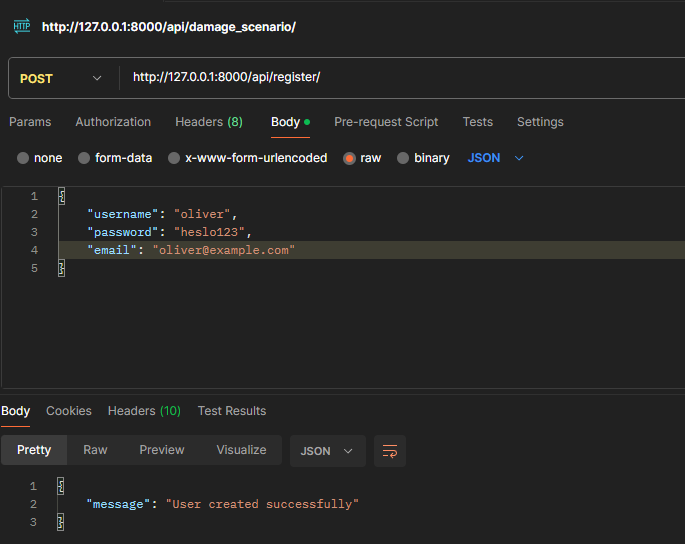
\includegraphics[width=\textwidth]{backend/scr1.png}
    \end{figure}
    \item Prihlásenie uživateľa - v odpovedi je token, ktorý sa použije v každej ďalšej požiadavke
    \begin{figure}[H]
        \centering
        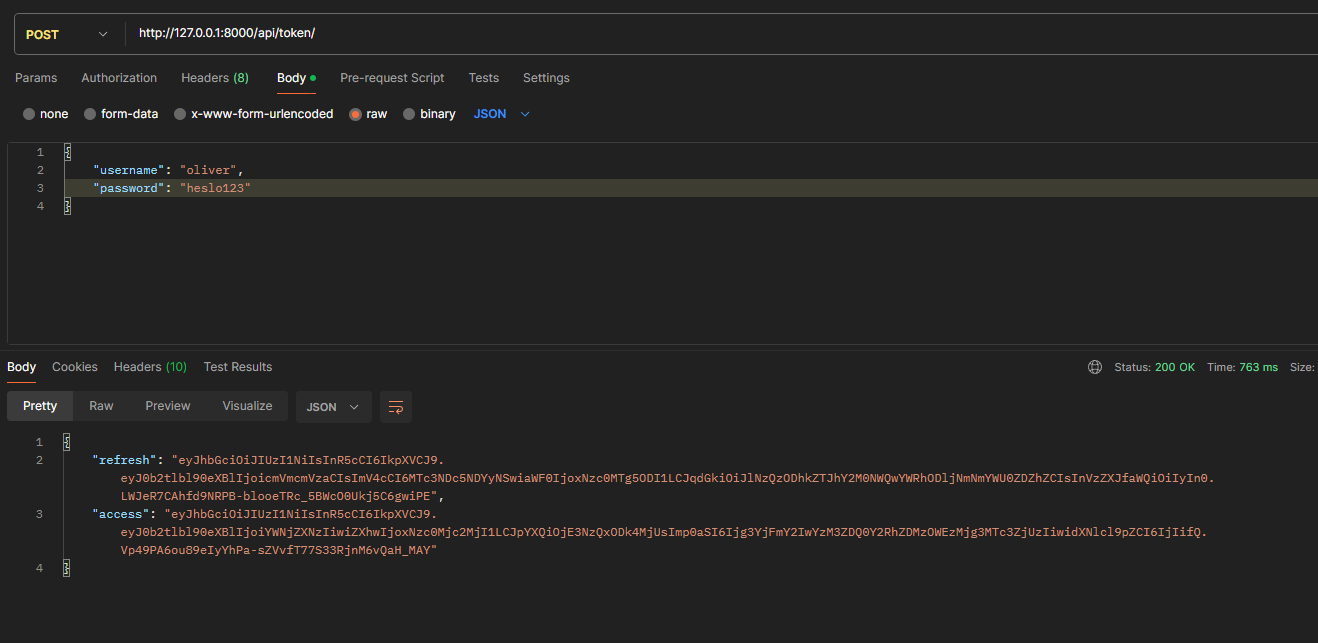
\includegraphics[width=\textwidth]{backend/scr2.png}
    \end{figure}
    \item Vytvorenie projektu. Na druhom obrázku je zobrazené, že token získaný v minulom kroku je v hlavičke \texttt{Authorisation}. Bude sa odosielať po celý zvyšok sedenia. Vytvorený projekt je takto asociovaný s daným uživateľom, a akékoľvek operácie s projektom budú musieť byť iba od tohto uživateľa.
    \begin{figure}[H]
        \centering
        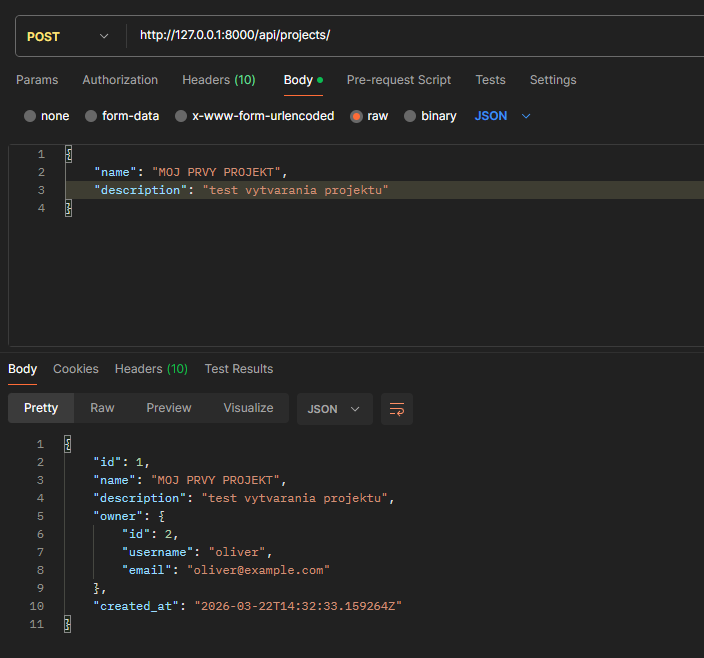
\includegraphics[width=\textwidth]{backend/scr3.png}
    \end{figure}
    \begin{figure}[H]
        \centering
        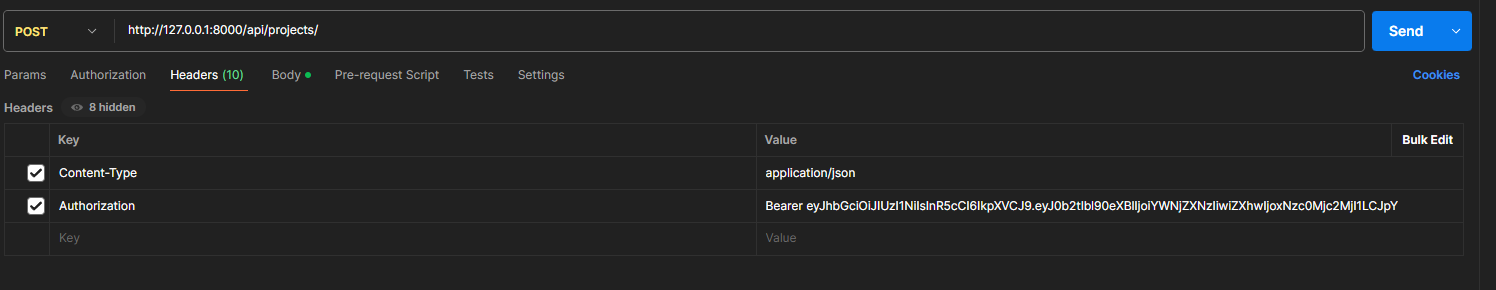
\includegraphics[width=\textwidth]{backend/scr4.png}
    \end{figure}
    \item Vytvorenie komponentu. Tu je dôležitá hlavne nová položka: \texttt{project\_id}. Komponent je teda asociovaný s práve jedným projektom. Táto položka, spolu s hlavičkou \texttt{Authorisation} bude v každej ďalšej požiadavke pracujúcej s projektom.
    \begin{figure}[H]
        \centering
        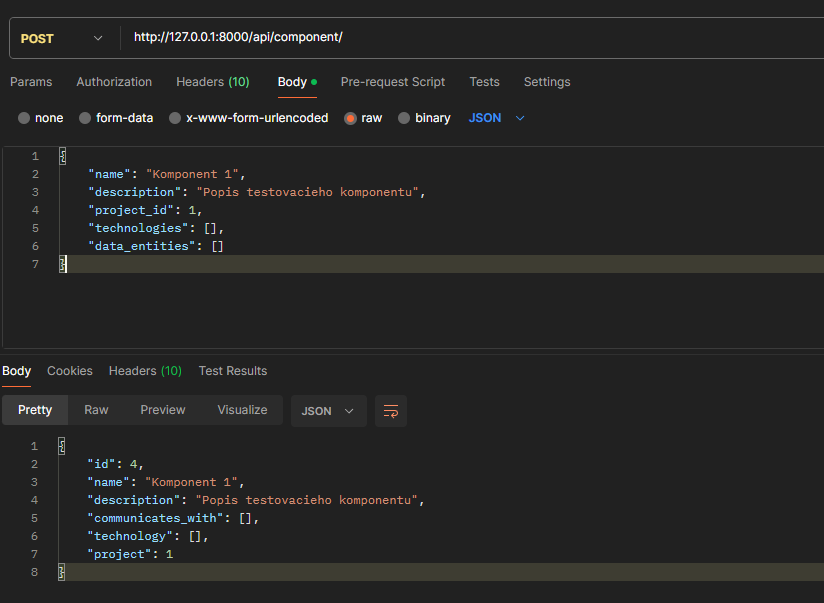
\includegraphics[width=\textwidth]{backend/scr5.png}
    \end{figure}
    \item Získanie zoznamu komponentov. V prípade GET požiadavky je číslo projektu v query parametroch (telo požiadavky na tomto obrázku je bezpredmetné, keďže ide o GET požiadavku). 
    \begin{figure}[H]
        \centering
        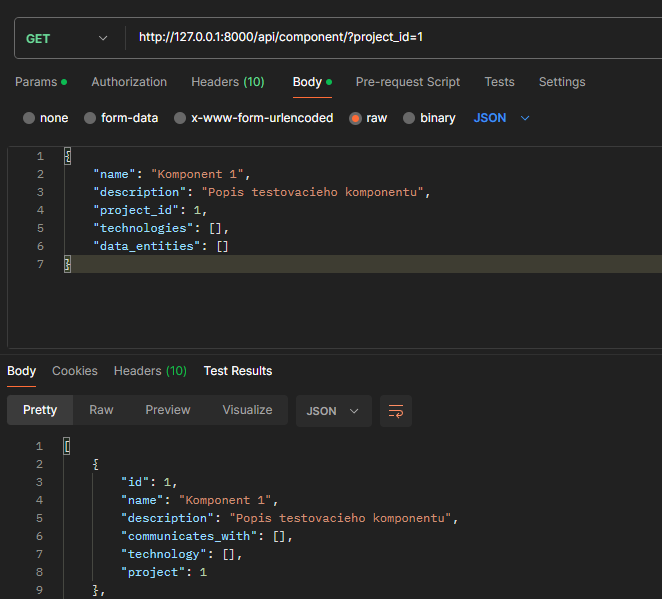
\includegraphics[width=\textwidth]{backend/scr6.png}
    \end{figure}
    \item Získanie detailov konkrétneho komponentu. V tomto prípade je v query URL číslo komponentu (tak ako v predošlej verzii API), a následne v query parametroch je číslo projektu (tak ako v predošlej požiadavke)
    \begin{figure}[H]
        \centering
        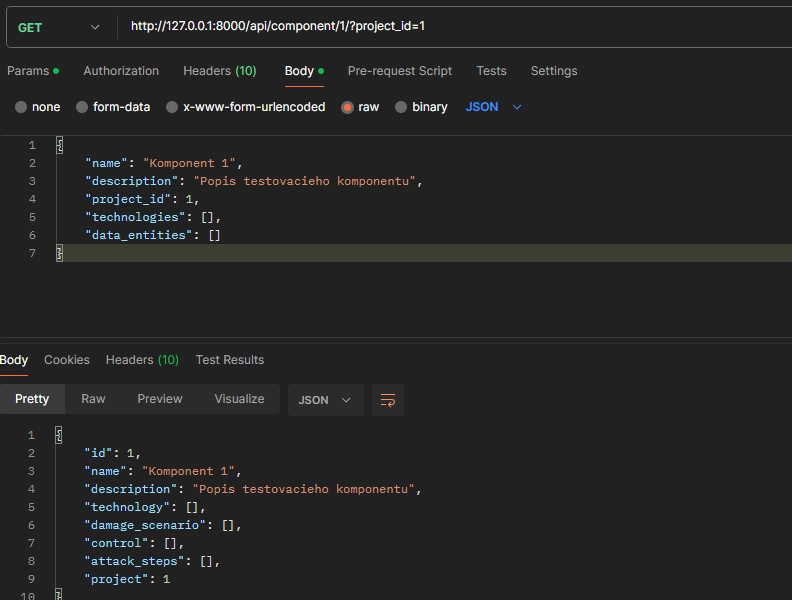
\includegraphics[width=\textwidth]{backend/scr7.png}
    \end{figure}
    \item Vytvorenie damage scenaria. Súčasťou tela požiadavky je \texttt{component\_id} a \texttt{project\_id}. Tým pádom je daný damage scenario asociovaný s práve jedným komponenom, ktorý je v práve jednom projekte, pričom ako už bolo spomenuté, vlastníctvo daného projektu uživateľom je zabezpečené hlavičkou \texttt{Authorisation}´. Na rovnakom princípe fungujú aj ostatné POST operácie, ako vytvorenie attack path alebo threat scenario.
    \begin{figure}[H]
        \centering
        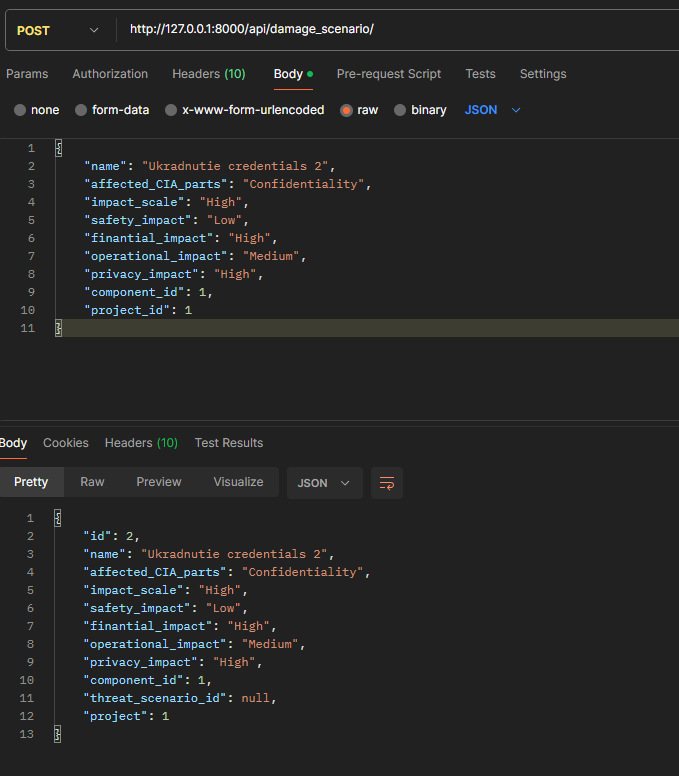
\includegraphics[width=\textwidth]{backend/scr8.png}
    \end{figure}
    \item Získanie detailov konkrétneho komponentu. Rovnaké ako pred dvoma krokmi - je tu iba pre ukážku, akým spôsobom sa damage scenario vytvorený v predošlom kroku pridal do komponentu.
    \begin{figure}[H]
        \centering
        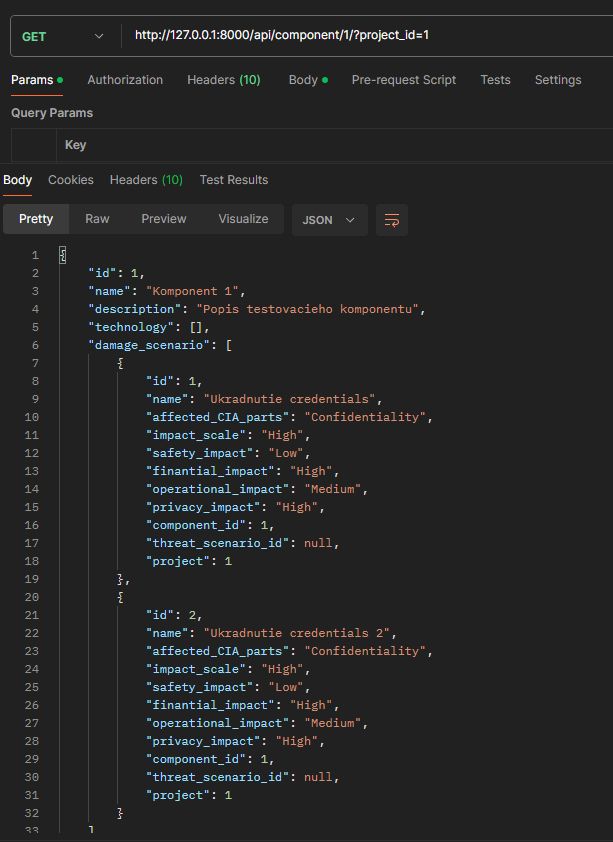
\includegraphics[width=\textwidth]{backend/scr9.png}
    \end{figure}
\end{enumerate}

Nové zmeny sú dostupné na rovnakom repozitári ako prototyp: \url{https://github.com/oldo7/TP_team12_backend}

\section{Výsledná implementácia}

Výsledkom projektu je funkčná webová aplikácia na tvorbu TARA analýzy pre automobilový systém. Aplikácia nie je iba jednoduchý formulár nad databázou, ale spája viacero spôsobov práce nad rovnakým modelom: grafický pohľad, tabuľkový pohľad, detailový editor, asistentov, konzolu s LLM návrhmi, výpočet rizík, prácu s control skupinami a export výsledného reportu do PDF. Hlavná myšlienka ostala rovnaká ako v návrhu -- uživateľ najprv vytvorí model systému, potom nad ním definuje damage scenarios, threat scenarios, attack steps a controls, a nakoniec vie vyhodnotiť riziká a pripraviť podklady pre mitigáciu.

Finálna implementácia je rozdelená na dve časti. Backend je vytvorený v technológii \texttt{Django} spolu s \texttt{Django REST Framework}. Stará sa o databázu, autorizáciu, kontrolu prístupu k projektom, výpočty TARA hodnôt, generovanie reportu a komunikáciu s LLM asistentom. Frontend je vytvorený v technológii \texttt{React} s nástrojom \texttt{Vite}. Na rozhranie používa knižnice \texttt{Tailwind}, \texttt{shadcn/ui}, \texttt{lucide-react}, \texttt{Zustand} a \texttt{@xyflow/react}. Frontend teda rieši hlavne prácu s uživateľom, vizualizáciu vzťahov, editáciu modelov a volanie backend API.

V nasledujúcich častiach je popísaná výsledná aplikácia tak, ako funguje po dokončení. Popis je písaný z pohľadu práce uživateľa, ale pri každej väčšej funkcionalite je zároveň uvedené, ako je riešená vnútri aplikácie a ako sú jednotlivé časti medzi sebou prepojené.

\subsection{Celkový tok práce v aplikácii}

Po otvorení aplikácie sa uživateľ najprv prihlási. Prihlásenie vyžaduje adresu backend servera, meno a heslo. Frontend predvolene očakáva backend na rovnakom hostiteľovi na porte \texttt{8000}, ale uživateľ môže adresu zmeniť. Ak uživateľ ešte nemá účet, môže na tej istej obrazovke prepnúť jednoduchý režim vytvorenia nového uživateľa. Po registrácii sa frontend rovno pokúsi prihlásiť s novým účtom. Po úspešnom prihlásení backend vráti dvojicu JWT tokenov -- \texttt{access} a \texttt{refresh}. Frontend si ich uloží do \texttt{sessionStorage} a následne ich používa pri každej požiadavke na backend.

Po prihlásení uživateľ vyberie existujúci projekt alebo vytvorí nový projekt. Projekt predstavuje samostatný TARA workspace. Všetky komponenty, technológie, scenáre, kroky útoku, controls a výsledné riziká sú vždy viazané na konkrétny projekt. Táto väzba je dôležitá aj bezpečnostne, pretože backend pri každom API volaní overuje, či prihlásený uživateľ skutočne vlastní projekt, ktorého sa požiadavka týka. Nestačí teda poznať \texttt{project\_id}; požiadavka musí mať aj platný JWT token pre vlastníka projektu.

Po výbere projektu sa otvorí hlavná pracovná plocha. Tá je rozdelená na tri hlavné režimy:

\begin{itemize}
    \item \textbf{Graph View} -- grafický pohľad, kde sú všetky modelové objekty zobrazené ako karty a vzťahy medzi nimi ako spojenia.
    \item \textbf{Table View} -- tabuľkový pohľad vhodný na rýchlu kontrolu scenárov, attack steps, controls, rizík a cybersecurity goals.
    \item \textbf{Assistants} -- asistenti, ktorí pomáhajú dopĺňať TARA model, napríklad identifikovať assets a vytvoriť základné damage/threat scenáre.
\end{itemize}

Tieto pohľady nepracujú s oddelenými dátami. Všetky používajú rovnaký stav projektu načítaný z backendu. Vo frontende je tento stav uložený v globálnom \texttt{Zustand} store. Store obsahuje mapy pre technológie, komponenty, data entities, controls, threat classes, attack steps, threat scenarios, damage scenarios, compromises a cybersecurity goals. Keď uživateľ niečo upraví v detailovom paneli alebo cez asistenta, zmena sa odošle do backendu a následne sa obnoví aj lokálny stav. Vďaka tomu sa rovnaká zmena prejaví v grafe, tabuľkách aj v detailoch.

Rozhranie hlavnej aplikácie má stabilné rozloženie. Hore je menubar a toolbar, vľavo je navigácia podľa aktuálneho režimu, v strede hlavný pracovný priestor, dole konzola a vpravo detailový panel. V hornom menu je okrem položiek \texttt{File} a \texttt{Help} aj tlačidlo \texttt{Login}, ktoré vymaže aktuálnu session, project ID a tokeny, a tým vráti aplikáciu späť na prihlasovaciu obrazovku. Toto je najjednoduchší spôsob, ako počas behu aplikácie prepnúť uživateľa. Toto rozloženie nadväzuje na pôvodný návrh aplikácie z kapitoly \uv{Návrh}, ale vo výslednej implementácii sú jednotlivé časti už funkčne prepojené.

\subsection{Autentizácia, projekty a prístupové práva}

Autentizácia je implementovaná pomocou JWT tokenov cez knižnicu \texttt{djangorestframework-simplejwt}. Backend poskytuje endpointy \texttt{/api/register/}, \texttt{/api/token/} a \texttt{/api/token/refresh/}. Registrácia vytvorí nového uživateľa v štandardnom Django modeli \texttt{User}. Vo frontende je registrácia dostupná priamo z prihlasovacej obrazovky cez možnosť \uv{Create a new user}. Uživateľ zadá meno, heslo a prípadne email. Po úspešnej registrácii frontend zavolá bežné prihlásenie, takže uživateľ nemusí manuálne prechádzať späť na login. Prihlásenie vráti access token a refresh token. Frontend access token posiela v hlavičke:

\begin{verbatim}
Authorization: Bearer <accessJWT>
\end{verbatim}

Každý projekt je uložený v modeli \texttt{Project}. Má názov, popis, vlastníka a dátum vytvorenia. Model projektu je jednoduchý, ale je centrálnym bodom celej aplikácie, pretože všetky ostatné projektové objekty majú na projekt cudzie kľúče alebo sú naň nepriamo naviazané.

Backend používa pomocnú funkciu \texttt{check\_project\_access}. Tá sa volá v jednotlivých endpointoch a kontroluje, či existuje projekt s daným ID a či jeho \texttt{owner} je aktuálne prihlásený uživateľ. Ak projekt neexistuje alebo nepatrí danému uživateľovi, backend vráti chybu \texttt{403}. Toto je použité konzistentne pri komponentoch, scenároch, control skupinách, rizikách, reportoch aj LLM asistentovi.

Vo frontende sa projekt vyberá na stránke \texttt{ProjectSelector}. Tá po prihlásení načíta zoznam projektov cez \texttt{/api/projects/}. Uživateľ môže projekt vybrať alebo rovno vytvoriť nový. ID a meno vybraného projektu sa uložia do \texttt{sessionStorage}. Po otvorení projektu komponent \texttt{ProjectPage} zavolá \texttt{loadProjectState}, čím sa naraz načíta celý projektový model a vypočítané riziká.

Toto riešenie má praktickú výhodu: uživateľ nemusí v jednotlivých obrazovkách opakovane vyberať projekt. Frontend automaticky prikladá \texttt{project\_id} ku každému relevantnému API volaniu. Backend napriek tomu nikdy neverí iba frontendu, ale vlastníctvo projektu kontroluje sám.

\subsection{Dátový model výslednej aplikácie}

Finálna databázová vrstva je postavená okolo TARA pojmov. Oproti pôvodnému návrhu pribudli niektoré objekty a niektoré vzťahy boli upravené tak, aby lepšie podporovali grafický editor a výpočet rizík.

\subsubsection{Technológie}

Model \texttt{Technology} reprezentuje technológie použité v systéme. Technológia má názov, popis a projekt. K technológiám sa môžu pripájať komponenty aj data entities. V praxi sem patria napríklad CAN, Ethernet, Bluetooth, Cellular, FreeRTOS, AUTOSAR SecOC alebo kryptografické mechanizmy.

Technológie samy o sebe netvoria riziko, ale pomáhajú popísať prostredie, v ktorom komponent funguje. V LLM kontexte a v asistentoch sa používajú ako nápoveda pre to, aké typy hrozieb alebo útokov môžu byť relevantné. Vo frontende sa technológie zobrazujú v strome pod komponentmi, v grafickom pohľade ako samostatné karty a v detailoch ako vzťahy.

\subsubsection{Komponenty}

Model \texttt{Component} reprezentuje časti analyzovaného systému. Komponent má názov, popis, projekt, zoznam použitých technológií a vzťah \texttt{communicates\_with} na iné komponenty. Tento komunikačný vzťah je obojsmerný \texttt{ManyToMany} vzťah, ktorý slúži na modelovanie toho, ktoré komponenty medzi sebou komunikujú.

Komponent je v aplikácii jeden z najdôležitejších modelov, pretože veľká časť TARA objektov sa naň naväzuje. Data entity patria ku komponentom, attack steps sa vykonávajú na komponentoch, controls sa aplikujú na komponenty a threat scenarios môžu obsahovať viacero komponentov. Backend má pri komponente aj odvodené vlastnosti \texttt{mapped\_threat\_scenarios} a \texttt{mapped\_damage\_scenarios}. Tie nezapisujú nové dáta do databázy, ale vypočítavajú, ktoré threat scenarios a damage scenarios sú s komponentom spojené cez existujúce vzťahy.

\subsubsection{Data entities}

Model \texttt{DataEntity} slúži na reprezentáciu dát, ktoré majú v systéme hodnotu. Data entity má názov, popis, voliteľný komponent, zoznam technológií a projekt. V aktuálnej implementácii sa data entities používajú hlavne ako assets pri asistente Asset Identification. Asistent prechádza data entities a komponenty, a pre každé z nich navrhuje možné straty Confidentiality, Integrity a Availability.

V pôvodnom návrhu boli data entities samostatným pilierom definície systému. Vo výslednej implementácii sú podporené v dátovom modeli aj vo frontende, ale hlavná TARA stopa je vo finále vedená najmä cez komponenty, damage scenarios, threat scenarios a attack steps.

\subsubsection{Threat classes}

Model \texttt{ThreatClass} reprezentuje triedu hrozby. Má názov, popis, voliteľné MITRE tactic ID a meno taktiky. Threat class sa dá priradiť k attack stepu alebo threat scenariu. Tým vzniká jednoduché prepojenie medzi vlastným TARA modelom a externou MITRE terminológiou.

Na strane backendu sú k dispozícii aj endpointy \texttt{/api/mitre/tactics/} a \texttt{/api/mitre/techniques/}. Tieto endpointy získavajú dáta z MITRE ATT\&CK STIX zdroja a poskytujú ich frontendu. Vo formulári pre threat class a attack step sa tak dajú používať MITRE taktiky a techniky bez toho, aby ich uživateľ musel manuálne prepisovať.

\subsubsection{Attack steps}

Model \texttt{AttackStep} popisuje konkrétny krok útoku. Má názov, popis, požadovaný prístup, komponent, threat class, MITRE technique ID a názov techniky. Dôležitou časťou sú hodnoty \texttt{fr\_et}, \texttt{fr\_se}, \texttt{fr\_koC}, \texttt{fr\_WoO} a \texttt{fr\_eq}. Tieto hodnoty reprezentujú faktory attack feasibility:

\begin{itemize}
    \item \textbf{Elapsed Time} -- čas potrebný na prípravu alebo vykonanie útoku.
    \item \textbf{Specialist Expertise} -- úroveň odbornosti útočníka.
    \item \textbf{Knowledge of Component} -- úroveň znalosti komponentu alebo systému.
    \item \textbf{Window of Opportunity} -- dostupnosť príležitosti na útok.
    \item \textbf{Equipment} -- potrebné vybavenie.
\end{itemize}

Attack step môže mať predchádzajúce kroky cez vzťah \texttt{previous\_steps}. Tento vzťah je orientovaný a umožňuje vytvoriť attack path. Ak napríklad útok vyžaduje najprv získanie fyzického prístupu a až potom flashovanie firmware, druhý krok môže mať prvý krok ako \texttt{previous\_step}. Backend pri výpočte threat scenaria potom nevníma attack steps iba ako nezávislý zoznam, ale snaží sa z nich vytvoriť možné cesty.

\subsubsection{Threat scenarios}

Model \texttt{ThreatScenario} spája komponenty, attack steps a damage scenarios. Threat scenario odpovedá na otázku, aká hrozba môže viesť k damage scenariu a cez ktoré attack steps sa dá realizovať. Má názov, popis, zoznam komponentov, zoznam attack steps, threat class a zoznam damage scenarios.

V implementácii je threat scenario veľmi dôležitý spojovací objekt. Ak attack step nie je priradený k threat scenariu, nevstupuje do výpočtu rizika. Ak damage scenario nie je priradené k threat scenariu, tiež nevzniká risk row. Preto backend aj frontend pri vytváraní vzťahov často automaticky dopĺňajú opačné väzby. Napríklad ak sa attack step pripojí k threat scenariu, backend zároveň vie zabezpečiť, aby komponent attack stepu bol pridaný medzi komponenty threat scenaria.

Threat scenario má aj súvisiaci model \texttt{Comporomises}. Názov modelu obsahuje preklep, ale v aplikácii funguje ako compromise záznam. Ukladá komponent, threat scenario a CIA bitmask toho, čo je na danom komponente kompromitované. Vďaka tomu môže threat scenario presnejšie popísať, či ide o stratu Confidentiality, Integrity alebo Availability na konkrétnej časti systému.

\subsubsection{Damage scenarios a concerns}

Model \texttt{DamageScenario} opisuje následok úspešného útoku. Má názov, popis, CIA bitmask, štyri impact hodnotenia a projekt. Štyri impact hodnotenia sú:

\begin{itemize}
    \item \textbf{safety\_impact}
    \item \textbf{finantial\_impact}
    \item \textbf{operational\_impact}
    \item \textbf{privacy\_impact}
\end{itemize}

V modeli je pole \texttt{impact\_scale}, ale vo výslednej implementácii sa nastavuje automaticky v metóde \texttt{save}. Hodnota \texttt{impact\_scale} je maximum zo štyroch impact kategórií. To znamená, že uživateľ nemusí ručne udržiavať dve konzistentné hodnoty. Stačí nastaviť safety, financial, operational a privacy impact a backend vypočíta celkový impact level.

CIA je uložená ako 3-bitová hodnota. Bit \texttt{4} znamená Confidentiality, bit \texttt{2} znamená Integrity a bit \texttt{1} znamená Availability. Kombinácie sú súčtom týchto hodnôt. Napríklad hodnota \texttt{7} znamená CIA, hodnota \texttt{6} znamená C+I a hodnota \texttt{1} znamená iba Availability. Backend aj frontend majú pomocné funkcie na prevod tejto hodnoty na čitateľný text.

Dôležitým rozšírením sú \texttt{DamageScenarioConcern}. Damage scenario už nemusí mať iba jednu globálnu CIA hodnotu. Concern hovorí, ktorého komponentu sa damage scenario týka a ktorá CIA časť je na ňom zasiahnutá. Backend povoľuje concerns iba pre komponenty, ktoré sú dostupné cez threat scenarios pripojené k danému damage scenariu. Ak sa zmenia vzťahy threat scenaria, backend neplatné concerns odstráni. Tým sa zabraňuje tomu, aby damage scenario odkazovalo na komponent, ktorý už s ním logicky nesúvisí.

Súhrnná CIA hodnota na damage scenariu sa synchronizuje z concerns. Ak má damage scenario viac concerns, backend spraví bitový súčet všetkých CIA častí. Uživateľ teda môže v detailovom paneli označiť napríklad Confidentiality na jednom komponente a Integrity na druhom komponente, a damage scenario bude mať súhrnne C+I.

\subsubsection{Controls a control classes}

Model \texttt{Control} reprezentuje bezpečnostné opatrenie. Control má názov, popis, voliteľnú control class, attack feasibility faktory, komponent, attack steps, threat scenarios a projekt. Na rozdiel od attack stepu tieto faktory nepopisujú útok samotný, ale dodatočnú náročnosť, ktorú control pridáva útočníkovi. Ak control napríklad vyžaduje obídenie kryptografickej autentizácie alebo získanie špeciálneho vybavenia, jeho hodnoty sa pripočítajú k hodnotám attack stepu.

Model \texttt{ControlClass} slúži ako šablóna pre controls. Obsahuje názov, popis a defaultné hodnoty faktorov. V databáze sú seedované preddefinované control classes. Vo formulári pre control si uživateľ môže vybrať triedu, čím sa automaticky vyplnia faktorové polia. Hodnoty sa však dajú ďalej upraviť, takže class slúži ako štartovací bod, nie ako pevné obmedzenie.

Controls môžu byť pripojené k attack steps aj k threat scenarios. Väzba na attack steps ovplyvňuje výpočet efektívnej attack feasibility. Väzba na threat scenarios slúži najmä na traceability, aby bolo jasné, ktorú hrozbu control adresuje. Vo formulári je to aj explicitne uvedené -- väzba na threat scenarios sama o sebe nemení výpočty.

\subsubsection{Control groups}

Model \texttt{ControlGroup} umožňuje vytvárať kombinácie controls. Skupina má názov, popis, projekt a zoznam controls. Aplikácia má aj dve virtuálne skupiny, ktoré nie sú uložené v databáze:

\begin{itemize}
    \item \textbf{All Controls} -- všetky controls v projekte sú aktívne.
    \item \textbf{No Controls} -- žiadne controls nie sú aktívne, zobrazuje sa základný stav bez mitigácie.
\end{itemize}

Uživateľ môže vytvoriť vlastnú skupinu, napríklad \uv{Minimal controls}, \uv{Production controls} alebo \uv{Proposed controls}. Vybraná skupina je uložená v \texttt{sessionStorage} a frontend ju používa pri zobrazovaní efektívnych AFL a RL hodnôt. Backend report zároveň obsahuje porovnanie control scenárov, kde pre každý risk ukazuje základný stav a stav pre jednotlivé control groups.

\subsubsection{Risk treatment a cybersecurity goals}

Model \texttt{RiskTreatment} ukladá rozhodnutie pre dvojicu threat scenario + damage scenario. Podporované rozhodnutia sú \texttt{avoid}, \texttt{reduce}, \texttt{share} a \texttt{accept}. Okrem rozhodnutia obsahuje aj textové odôvodnenie. V tabuľke risks vie uživateľ priamo otvoriť detail rizika a zapísať treatment podľa ISO/SAE 21434.

Model \texttt{CybersecurityGoal} reprezentuje cybersecurity goal. Má názov, popis, voliteľnú hodnotu CAL od 1 do 4, zoznam damage scenarios, zoznam controls a projekt. V aplikácii sa tým uzatvára stopa od damage scenaria cez riziko až po bezpečnostný cieľ a opatrenia, ktoré ho adresujú.

\subsection{Výpočet attack feasibility, impact a risk level}

Výpočtová logika je oddelená v súbore \texttt{calculations.py}. Táto časť je dôležitá, lebo z modelovaných objektov robí TARA analýzu.

Attack feasibility sa počíta z piatich faktorov attack stepu:

\begin{verbatim}
points = fr_et + fr_se + fr_koC + fr_WoO + fr_eq
\end{verbatim}

Ak je \texttt{fr\_et} alebo \texttt{fr\_WoO} nastavené na \texttt{99}, výsledok sa berie ako \uv{Not practical}. Vtedy sa attack potential body nezobrazujú ako číslo a AFL sa nastaví na veľmi nízku uskutočniteľnosť útoku.

Inak sa body mapujú na attack potential a AFL:

\begin{itemize}
    \item 0 až 9 bodov: \textbf{Basic}, AFL \textbf{High}, hodnota 5.
    \item 10 až 13 bodov: \textbf{Enhanced-Basic}, AFL \textbf{High}, hodnota 4.
    \item 14 až 19 bodov: \textbf{Moderate}, AFL \textbf{Medium}, hodnota 3.
    \item 20 až 24 bodov: \textbf{High}, AFL \textbf{Low}, hodnota 2.
    \item viac ako 24 bodov: \textbf{Beyond High}, AFL \textbf{Very Low}, hodnota 1.
\end{itemize}

Táto logika je použitá pre attack steps aj pre controls. Pri attack stepe hodnoty reprezentujú náročnosť samotného útoku. Pri controle hodnoty reprezentujú dodatočnú náročnosť na obídenie daného opatrenia.

Impact level sa počíta ako maximum zo safety, financial, operational a privacy impact hodnoty. Hodnoty sú uložené ako číselné voľby:

\begin{itemize}
    \item 0 -- Negligible
    \item 1 -- Moderate
    \item 2 -- Major
    \item 3 -- Severe
\end{itemize}

Risk level sa počíta z impact level a AFL hodnoty pomocou matice \texttt{RISK\_LEVEL\_MATRIX}. Výsledkom je hodnota 1 až 5. Ak threat scenario nemá žiadny attack step, AFL nie je známe a risk level sa nedá vypočítať.

Pri threat scenariu sa attack feasibility nepočíta iba jednoduchým minimom alebo maximom všetkých attack steps. Backend najprv vytvorí možné attack paths z \texttt{previous\_steps}. Ak kroky tvoria orientovaný graf, vyhľadá všetky cesty od koreňových krokov po listy. Každá cesta je obmedzená svojím najťažším krokom, teda bottleneckom. Útočník si potom vyberá najľahšiu kompletnú cestu. Implementačne sa pre každú cestu vyberie najhoršie hodnotený krok a následne sa z týchto bottleneckov vyberie pre útočníka najvýhodnejší. Ak kroky nemajú poradie, každý krok sa berie ako samostatná cesta.

Pri aktívnych controls sa používa podobná logika, ale pre každý attack step sa najprv vypočíta efektívna attack feasibility. Frontend aj backend berú relevantné iba tie controls, ktoré sú pripojené k danému attack stepu. Ich hodnoty sa pripočítajú k základným hodnotám attack stepu. Tým sa vie ukázať rozdiel medzi základným rizikom a rizikom po aplikovaní control skupiny.

\subsection{Backend API a synchronizácia vzťahov}

Backend API má klasické CRUD endpointy pre hlavné modely: technologies, components, damage scenarios, controls, attack steps, threat scenarios, threat classes, control groups, cybersecurity goals a projekty. Okrem toho poskytuje endpointy pre výpočet rizík, risk treatment, report, MITRE dáta a LLM asistenta.

Jednotlivé endpointy používajú serializéry z \texttt{serializers.py}. Serializéry nerobia iba jednoduché mapovanie databázových polí. Obsahujú aj spätnú kompatibilitu pre staršie textové hodnoty. Napríklad impact hodnoty môžu byť zadané ako čísla, ale aj ako slová typu \texttt{low}, \texttt{medium}, \texttt{high}, \texttt{critical}. Podobne CIA bitmask vie spracovať hodnoty ako \texttt{C}, \texttt{I}, \texttt{A}, \texttt{CIA}, \texttt{111} alebo číselné hodnoty. Vďaka tomu je API tolerantnejšie a lepšie sa používa aj z LLM návrhov alebo z testovacích nástrojov.

V endpointoch je viacero synchronizačných helperov. Funkcia \texttt{sync\_threat\_scenarios} sa používa napríklad pri attack stepoch a controls. Ak sa vytvára objekt s názvom threat scenaria alebo so zoznamom threat scenarios, backend zabezpečí správne prepojenie. Ak má attack step komponent, komponent sa doplní aj do threat scenaria. Podobne \texttt{sync\_threat\_scenario\_components} zjednocuje komponenty threat scenaria podľa priamych komponentov, komponentov z attack steps a komponentov z compromise záznamov.

Pri damage scenarios sa používa \texttt{sync\_damage\_scenario\_concerns}. Tá kontroluje, či každý concern odkazuje na komponent, ktorý je povolený cez pripojené threat scenarios. Neplatné concerns sú odstránené. Následne sa z concerns vypočíta súhrnná CIA hodnota. Toto riešenie udržiava model konzistentný aj pri postupnej editácii z grafu, tabuľky alebo detailového panelu.

Frontend nad týmto API používa všeobecné funkcie \texttt{createModel}, \texttt{updateModel} a \texttt{deleteModel}. Tie podľa typu objektu vedia zavolať správny endpoint. Pri vytváraní objektov frontend pridáva \texttt{project\_id} z aktuálneho projektu. Pri editácii sa zmeny ukladajú automaticky z detailového panelu s oneskorením 500 ms, aby sa pri písaní neposielala požiadavka po každom stlačení klávesy.

\subsection{Grafický pohľad}

Grafický pohľad je hlavný spôsob práce s modelom. Je implementovaný cez knižnicu \texttt{@xyflow/react}. Každý modelový objekt sa zobrazuje ako karta. Karta obsahuje názov, krátky popis, typ objektu a niekoľko metadát podľa typu. Napríklad komponent ukazuje počet komunikačných vzťahov a technológií, damage scenario ukazuje CIA a IL, attack step ukazuje komponent a počet threat scenarios, control ukazuje komponent a počet mitigovaných attack steps.

Graf sa skladá z uzlov a hrán. Uzly vznikajú zo všetkých modelových máp v lokálnom store. Z grafu sú momentálne vynechané cybersecurity goals, pretože tie sú lepšie čitateľné v tabuľkovom pohľade a detailoch. Hrany vznikajú z reálnych vzťahov medzi objektmi:

\begin{itemize}
    \item komponent komunikuje s komponentom,
    \item komponent používa technológiu,
    \item data entity patrí ku komponentu alebo používa technológiu,
    \item control patrí ku komponentu,
    \item attack step patrí ku komponentu,
    \item attack step je prepojený s controls,
    \item attack step nadväzuje na predchádzajúci attack step,
    \item attack step alebo threat scenario majú threat class,
    \item threat scenario obsahuje komponenty, attack steps a damage scenarios,
    \item damage scenario je späť prepojené s threat scenarios,
    \item compromise odkazuje na komponent a threat scenario.
\end{itemize}

Uživateľ môže karty presúvať po ploche. Pozície sa ukladajú do \texttt{localStorage} pod kľúčom odvodeným od projektu. V menu \texttt{File} je možné layout uložiť do JSON súboru a neskôr ho načítať. Po načítaní layoutu frontend nastaví uložené pozície na existujúce uzly.

Graf podporuje aj filtrovanie. Uživateľ môže filtrovať podľa názvu a podľa typu objektu. Filtrovanie ovplyvňuje iba zobrazenie grafu, nie dáta v projekte. Pri kliknutí na kartu sa vybraný objekt nastaví ako \texttt{selectedItem} a otvorí sa v pravom detailovom paneli. Ak uživateľ vyberie objekt v strome, graf sa naň vie automaticky centrovať.

Dôležitá funkcionalita je vytváranie spojení priamo v grafe. Každá karta má connection handles. Pri spojení dvoch kariet frontend zistí typ zdrojového a cieľového objektu a cez funkciu \texttt{isConnectable} overí, či medzi nimi existuje povolený vzťah. Ak áno, zavolá \texttt{addConnection}. Tá nájde správny smer vzťahu a správne pole. Napríklad pri spojení attack stepu s threat scenariom sa upraví zoznam \texttt{threat\_scenarios} na attack stepe alebo zoznam \texttt{attack\_steps} na threat scenariu podľa toho, ktorá strana vlastní daný vzťah v dátovom modeli.

Týmto spôsobom môže uživateľ model skladať vizuálne. Nemusí si pamätať ID objektov ani manuálne editovať všetky zoznamy vzťahov. Aplikácia zároveň zabraňuje duplicitnému prepojeniu a nepovolí vzťahy, ktoré dátový model nepodporuje.

\subsection{Strom projektu a vytváranie súvisiacich objektov}

Ľavý panel v grafickom režime obsahuje strom projektu. Strom je načítaný z backendu cez funkciu \texttt{getProjectTree}. Zobrazuje komponenty a pod nimi súvisiace technológie, damage scenarios, attack steps, threat scenarios a ďalšie odkazy. Strom má vyhľadávanie, takže pri väčšom projekte sa dá rýchlo nájsť konkrétny scenár alebo komponent.

Strom funguje aj ako navigácia. Kliknutím na položku sa nastaví vybraný objekt. Detailový panel ho otvorí na editáciu a graf sa naň môže zamerať. Ak je vybraný objekt, v strome sa zobrazí tlačidlo na pridanie súvisiaceho modelu. Po kliknutí sa otvorí dialóg, v ktorom sa dá buď vybrať existujúci objekt a pripojiť ho, alebo vytvoriť nový objekt a hneď ho pripojiť k aktuálne vybranému.

Tento istý princíp je použitý aj v detailovom paneli. Vzťahy nie sú zobrazené iba ako text. Sú to klikateľné značky, ktoré umožňujú rýchlo prejsť na súvisiaci objekt. Vedľa zoznamu vzťahov je tlačidlo na pridanie ďalšieho vzťahu. Uživateľ teda môže začať napríklad na komponente, vytvoriť k nemu attack step, z attack stepu vytvoriť threat scenario, k threat scenariu pridať damage scenario a potom vrátiť sa k attack stepu a doplniť controls.

\subsection{Detailový panel a formuláre}

Pravý panel je detailový editor. Jeho obsah závisí od typu vybraného modelu. Pre jednoduché objekty, ako technológia, komponent alebo data entity, obsahuje hlavne názov a popis. Pre TARA objekty obsahuje špecifické polia.

Pri damage scenariu sa zobrazuje názov, popis, affected components, CIA checkboxy a impact hodnoty. CIA sa zadáva cez checkboxy pre Confidentiality, Integrity a Availability. Ak damage scenario má pripojené threat scenarios, formulár vie odvodiť komponenty, ktoré môžu byť affected. Uživateľ potom nastavuje CIA na úrovni konkrétnych komponentov. Formulár zároveň ukazuje vypočítaný IL.

Pri attack stepe sa zadáva názov, popis, required access, MITRE technika, threat class a všetky attack feasibility faktory. Formulár obsahuje aj niekoľko praktických príkladov, napríklad CAN frame injection, diagnostic service abuse, firmware extraction alebo credential/key compromise. Výber príkladu predvyplní názov, popis, required access a faktorové hodnoty. Uživateľ si ich vie upraviť podľa konkrétneho projektu.

Pri controle formulár obsahuje názov, popis, výber control class, pripojené threat scenarios a faktorové hodnoty. Ak uživateľ vyberie control class, frontend preberie jej defaultné hodnoty. Pod hodnotami sa zobrazuje aj vypočítaná attack feasibility controlu. Pri attack stepe sa navyše zobrazuje efektívne AFL s aktívnymi controls, ak je vybraná control skupina a daný step má relevantné controls.

Pri threat scenariu sa zadáva názov, popis, threat class a involved components. Aj tu sú dostupné príklady, napríklad spoofed in-vehicle network messages, unauthorized diagnostic access, malicious software update alebo remote service exploitation. Pri cybersecurity goal sa nastavuje názov, popis, CAL a väzby na damage scenarios a controls.

Detailový panel teda nie je len prezeranie dát. Je to hlavný editor, ktorý umožňuje priebežne ukladať zmeny, mazať objekty, pridávať vzťahy a prechádzať medzi súvisiacimi časťami modelu.

\subsection{Tabuľkový pohľad}

Tabuľkový pohľad je určený na kontrolu a analýzu. Vľavo má navigáciu medzi tabuľkami a pri každej tabuľke zobrazuje počet položiek. Implementované tabuľky sú:

\begin{itemize}
    \item Threat Scenarios,
    \item Damage Scenarios,
    \item Attack Steps,
    \item Controls,
    \item Risks,
    \item Cybersecurity Goals.
\end{itemize}

Každá tabuľka má hlavné stĺpce, ktoré dávajú prehľad o danom type objektu. Riadky sú klikateľné. Kliknutím sa jednak nastaví vybraný objekt v detailovom paneli a jednak sa riadok rozbalí. Rozbalená časť obsahuje detailnejšie informácie, napríklad popis, súvisiace komponenty, zoznam attack steps, impact hodnoty alebo attack feasibility faktory.

Tabuľka damage scenarios ukazuje ID, názov, IL, CIA a threat scenarios. Po rozbalení ukazuje popis, impact detail a concerns. Tabuľka attack steps ukazuje komponent, threat scenarios a AFL. Ak je aktívna control skupina, tabuľka vie zobraziť efektívne AFL s controls a pôvodné základné AFL. Podobne tabuľka risks vie zobraziť efektívne RL, ak sa po aplikovaní controls zmení.

Tabuľka risks je najdôležitejšia pre výslednú analýzu. Backend endpoint \texttt{/api/risk/} vytvorí riadky na základe kombinácií threat scenarios a damage scenarios. Pre každý riadok vypočíta AFL, IL a RL. Ak damage scenario obsahuje concerns, vzniká riadok aj na úrovni konkrétneho affected komponentu. Ak ide o starší damage scenario bez concerns, endpoint vie stále vytvoriť legacy riadok zo súhrnnej CIA hodnoty.

V rozbalenom detaile risku je aj editor risk treatment. Uživateľ môže vybrať rozhodnutie Avoid, Reduce, Share alebo Accept a dopísať rationale. Uloženie zavolá endpoint \texttt{/api/risk\_treatment/}. Po uložení sa riziká znovu načítajú, aby tabuľka zobrazovala aktuálny treatment.

Tabuľkový pohľad má tlačidlo \texttt{New} pre tie tabuľky, kde dáva zmysel vytvárať nové objekty. Tým sa otvorí rovnaký formulárový dialóg ako v grafickom pohľade. Používanie aplikácie teda nie je viazané na jeden workflow. Uživateľ môže modelovať vizuálne alebo tabuľkovo podľa toho, čo je v danej chvíli prehľadnejšie.

\subsection{Control skupiny a porovnávanie mitigácií}

Control skupiny sú dostupné z toolbaru cez tlačidlo \texttt{Controls}. Dialóg zobrazuje dve vstavané skupiny \texttt{All Controls} a \texttt{No Controls}, a potom všetky uživateľské skupiny z databázy. Uživateľ môže skupinu vybrať, vytvoriť novú, upraviť existujúcu alebo ju zmazať.

Pri vytváraní alebo úprave skupiny sa zadáva názov, popis a zoznam controls. Výber aktívnej skupiny ovplyvňuje výpočty zobrazované vo frontende. Ak je aktívna skupina \texttt{No Controls}, attack steps a risks ukazujú základný stav. Ak je aktívna skupina \texttt{All Controls}, aplikujú sa všetky controls, ktoré sú pripojené k attack steps. Pri vlastnej skupine sa aplikujú iba vybrané controls.

Technicky sa aktívna skupina ukladá vo \texttt{Zustand} store ako hodnota \texttt{activeControlGroupId}. Môže to byť \texttt{all}, \texttt{none} alebo ID reálnej skupiny. Funkcia \texttt{getActiveControlIds} podľa toho vráti zoznam aktívnych control ID. Tento zoznam potom používajú výpočty v tabuľkách a formulároch.

Na backendu sa control groups ukladajú v modeli \texttt{ControlGroup}. Report generátor ich používa na samostatnú tabuľku \uv{Control Scenarios per Risk}. Tam sa pre každý risk ukáže základný risk level a risk level pri jednotlivých control skupinách. To je užitočné najmä pri porovnávaní alternatívnych mitigácií. Uživateľ vie napríklad ukázať, že minimálna sada opatrení zníži RL z 4 na 3, ale plná sada opatrení zníži RL z 4 na 2.

\subsection{Asset Identification assistant}

V režime \texttt{Assistants} je implementovaný asistent \texttt{Asset Identification}. Jeho cieľom je pomôcť uživateľovi vytvoriť základné damage a threat scenarios pre existujúce assets. Asistent prechádza všetky data entities a komponenty v projekte. Pre každý asset vytvorí tri návrhy -- Confidentiality, Integrity a Availability.

Návrhy sa zobrazujú v tabuľkovom zozname. Pri každom návrhu je stav: Proposed, Accepted, Rejected alebo Creating. Uživateľ môže návrh prijať, odmietnuť, obnoviť odmietnutý návrh alebo použiť \texttt{Apply All}. Pri jednom assete sa dá použiť aj \texttt{Apply All} iba pre jeho tri CIA časti.

Keď uživateľ prijme návrh, frontend vytvorí nové threat scenario a nové damage scenario. Threat scenario má názov typu \uv{Confidentiality compromise of ...} a description obsahuje interný source tag. Damage scenario má názov typu \uv{Loss of Confidentiality for ...}. Ak asset patrí ku komponentu, damage scenario dostane concern na daný komponent s príslušnou CIA hodnotou. Threat scenario je pripojené ku komponentu a damage scenario je pripojené k threat scenariu.

Source tag v popise nie je viditeľná funkcionalita pre koncového uživateľa, ale používa sa na rozpoznanie, či už bol návrh vytvorený. Asistent vie nájsť damage scenario, ktoré obsahuje rovnaký source tag, a potom ho zobrazí ako \uv{Created}. Zároveň vie nájsť aj existujúce scenáre, ktoré už pokrývajú rovnaký komponent a CIA časť, a vtedy namiesto \uv{Accept} zobrazí možnosť \uv{Add another}. Tým sa znižuje riziko, že asistent bude vytvárať duplicitné scenáre bez upozornenia.

Tento asistent je jednoduchší ako plný LLM asistent v konzole, ale má výhodu, že je deterministický. Nepotrebuje externé API a funguje vždy nad aktuálnym modelom. Je vhodný hlavne v začiatku analýzy, keď má projekt definované komponenty a dáta, ale ešte chýbajú základné damage scenarios.

\subsection{Konzola a LLM návrhy}

Spodný panel aplikácie obsahuje konzolu. Konzola pôvodne mala slúžiť ako história akcií, ale vo finálnej implementácii je zároveň komunikačným rozhraním s TARA asistentom. Uživateľ môže do nej napísať otázku, požiadať o analýzu aktuálneho modelu alebo požiadať o vytvorenie návrhov.

Frontend najprv odošle prompt na backend endpoint \texttt{/api/langchains/prepare/}. Spolu s promptom posiela históriu posledných správ a pamäť predchádzajúcich návrhov. Backend zostaví kontext projektu, ktorý obsahuje počty objektov, komponenty, technológie, damage scenarios, attack steps, threat scenarios, controls a mapu vzťahov. Tento kontext dá LLM modelu spolu so systémovým promptom.

Backend LLM časť je implementovaná v súboroch \texttt{langchains.py} a \texttt{langchain\_tools.py}. Používa \texttt{langchain-deepseek} a nástroje definované cez LangChain tools. Model môže zavolať napríklad:

\begin{itemize}
    \item \texttt{propose\_technology},
    \item \texttt{propose\_component},
    \item \texttt{propose\_damage\_scenario},
    \item \texttt{propose\_attack\_step},
    \item \texttt{propose\_threat\_scenario},
    \item \texttt{propose\_control},
    \item \texttt{analyze\_current\_state}.
\end{itemize}

Dôležité je, že LLM priamo nezapisuje do databázy. Nástroje iba pripravia návrhy. Každý návrh má \texttt{tempId}, typ, názov, popis, rationale, payload a prípadné references na iné návrhy. Frontend tieto návrhy zobrazí v dialógu \texttt{LangchainProposalDialog}. Uživateľ ich môže rozbaliť, skontrolovať a až potom jednotlivo prijať alebo odmietnuť.

Pri prijatí návrhu frontend zavolá \texttt{createLangchainProposal}. Tá podľa typu návrhu vytvorí príslušný objekt cez štandardné model API. Ak návrhy medzi sebou odkazujú cez dočasné references, frontend ich vie po vytvorení zosúladiť cez \texttt{reconcileAcceptedProposals}. To umožňuje napríklad situáciu, kde LLM v jednej odpovedi navrhne nový attack step, nové damage scenario a threat scenario, ktoré ich má prepojiť. Kým objekty ešte nemajú databázové ID, vzťahy sa držia cez temp IDs. Po prijatí sa nahradia reálnymi ID.

Konzola má aj lokálny fallback. Ak backend assistant nie je dostupný alebo nie je nakonfigurovaný, frontend vie spraviť jednoduchú lokálnu analýzu stavu alebo pripraviť lokálne draft návrhy. Pri analýze spočíta objekty a upozorní na medzery, napríklad komponent bez damage scenarios, komponent bez attack steps alebo komponent bez controls. Táto funkcionalita je užitočná pri vývoji a demonštrácii, pretože aplikácia ostáva použiteľná aj bez externého LLM providera.

LLM asistent si tiež pamätá stav návrhov. Ak uživateľ návrh prijal, odmietol alebo jeho uloženie zlyhalo, táto informácia sa posiela späť do backendu ako \texttt{proposalMemory}. Systémový prompt explicitne hovorí modelu, aby neopakoval už prijaté, odmietnuté alebo čakajúce návrhy, pokiaľ uživateľ nepožiada o ich revíziu. Tým sa zlepšuje použiteľnosť pri konverzačnej práci typu \uv{analyzuj model}, \uv{navrhni chýbajúce controls}, \uv{pokračuj}.

\subsection{MITRE integrácia}

Aplikácia obsahuje jednoduchú integráciu MITRE ATT\&CK. Backend má súbor \texttt{mitre.py}, ktorý načítava STIX bundle a poskytuje endpointy pre tactics a techniques. Frontend má funkcie \texttt{fetchMitreTactics} a \texttt{fetchMitreTechniques}, ktoré tieto dáta používajú vo formulároch.

V dátovom modeli sú MITRE väzby uložené priamo ako textové polia. Threat class má \texttt{mitre\_tactic\_id} a \texttt{mitre\_tactic\_name}. Attack step má \texttt{mitre\_technique\_id} a \texttt{mitre\_technique\_name}. Takéto riešenie je jednoduché a praktické. Aplikácia nemusí ukladať celý MITRE dataset do vlastnej databázy, ale zvolená taktika alebo technika ostane uložená pri konkrétnom TARA objekte.

MITRE teda vo výslednej aplikácii neslúži ako automatický generátor analýzy. Slúži skôr ako referenčná vrstva a slovník, ktorý pomáha pomenovať attack steps a threat classes konzistentne s existujúcou bezpečnostnou terminológiou.

\subsection{Generovanie PDF reportu}

Toolbar obsahuje tlačidlo \texttt{Generate Report}. Po kliknutí frontend zavolá endpoint \texttt{/api/report/} s \texttt{project\_id}. Backend overí prístup k projektu a zavolá funkciu \texttt{generate\_report\_pdf}. Výsledkom je PDF súbor, ktorý frontend stiahne ako \texttt{tara-report-<projectId>.pdf}.

Report je generovaný pomocou knižnice \texttt{reportlab}. Graf rizík sa generuje cez \texttt{matplotlib}. Report obsahuje viacero sekcií:

\begin{itemize}
    \item základné informácie o projekte,
    \item risk distribution chart,
    \item assets -- data entities,
    \item assets -- components,
    \item damage scenarios overview,
    \item cross-reference medzi damage a threat scenarios,
    \item threat scenarios and attack paths,
    \item attack steps table,
    \item controls table,
    \item risks table,
    \item control scenarios per risk,
    \item risk treatment table,
    \item cybersecurity goals.
\end{itemize}

Report používa rovnaké výpočty ako backend API. Threat scenarios sa prechádzajú spolu s attack steps a damage scenarios. Pre každú unikátnu dvojicu threat scenario + damage scenario sa vypočíta AFL, IL a RL. Potom sa tieto riadky používajú v risk tabuľke a v grafe rozloženia rizík.

Risk distribution chart zobrazuje maticu impact vs. attack feasibility. Farebné bunky zodpovedajú risk levelom a kruhy ukazujú počet rizík v jednotlivých bunkách. Tým report poskytuje rýchly vizuálny prehľad, či sa riziká sústreďujú v nízkych alebo vysokých oblastiach.

Sekcia control scenarios per risk porovnáva základný stav bez controls a všetky definované control groups. Pre každú control group backend znovu vypočíta efektívnu attack feasibility threat scenaria a z nej nový risk level. V PDF je tak vidno, ktoré opatrenia majú reálny vplyv na výsledné riziko.

Report je navrhnutý ako praktický výstup z aplikácie. Nemá nahrádzať všetku dokumentáciu TARA procesu, ale poskytuje export aktuálneho stavu projektu vo forme, ktorú je možné poslať, archivovať alebo použiť ako podklad pre ďalšiu diskusiu.

\subsection{Vzťah medzi grafom, tabuľkami, detailmi a backendom}

Jedna z najdôležitejších častí výslednej implementácie je, že aplikácia nemá tri oddelené editory. Graf, tabuľky a detailový panel sú tri rôzne pohľady na rovnaký model. Z technického pohľadu to zabezpečuje \texttt{model-store.ts}.

Pri otvorení projektu store zavolá \texttt{getProjectState} a \texttt{getProjectRisks}. Projektový stav sa uloží ako mapy podľa typu modelu. Riziká sa ukladajú ako pole \texttt{risks}. Komponenty, scenáre a controls sa potom používajú na tvorbu grafových uzlov, tabuľkových riadkov, formulárov aj zoznamov vzťahov.

Keď uživateľ upraví objekt v detailovom paneli, najprv sa zmení lokálny stav cez \texttt{setItem}. Po krátkom oneskorení sa zavolá \texttt{saveItem}, ktorý pošle update na backend. Ak ide o typ, ktorého zmena môže ovplyvniť vzťahy a riziká, napríklad threat scenario, damage scenario alebo attack step, frontend po uložení znovu načíta projektový stav. Tým sa aktualizujú odvodené polia, concerns, riziká aj strom.

Keď uživateľ vytvorí nový objekt, \texttt{addItem} ho uloží cez API. Ak API vráti objekt s projektom, frontend znovu načíta celý projektový stav. Je to jednoduchšie a bezpečnejšie ako ručne skladať všetky odvodené vzťahy na klientovi. Pri mazaní objektu sa volá \texttt{deleteItem}, ktorý zmaže objekt cez API a potom ho odstráni z lokálneho store.

Vzťahy sa spravujú cez \texttt{addConnection} a \texttt{deleteConnection}. Tieto funkcie najprv určia, ktorá strana vzťahu vlastní príslušné pole. Napríklad data entity má pole \texttt{component}, component nemá pole \texttt{data\_entities}. Pri vzťahu data entity -- component sa teda upravuje data entity. Pri many-to-many vzťahoch sa upravuje pole so zoznamom ID. Toto umožňuje, aby rovnaké vytváranie vzťahov fungovalo z grafu, zo stromu aj z detailového panelu.

\subsection{Príklad práce s aplikáciou}

Typický workflow môže vyzerať takto:

\begin{enumerate}
    \item Uživateľ sa prihlási a otvorí projekt \uv{Auto security}.
    \item V graph view vytvorí komponenty ako Infotainment Head Unit, Central Gateway, TCU alebo Engine ECU.
    \item Ku komponentom pripojí technológie ako CAN, Bluetooth/BLE, Cellular alebo Automotive Ethernet.
    \item V asistentovi Asset Identification pre komponenty alebo data entities prijme návrhy CIA strát. Tým sa vytvoria prvé threat scenarios a damage scenarios.
    \item V detailoch damage scenaria nastaví konkrétne affected components a impact hodnoty pre safety, financial, operational a privacy.
    \item Vytvorí attack steps, napríklad Gateway Firewall Bypass, Unauthorized Firmware Flashing alebo CAN Command Injection. Pri každom doplní faktorové hodnoty pre attack feasibility.
    \item Attack steps pripojí k threat scenarios a threat scenarios k damage scenarios. V grafe tým vznikne stopa od útoku cez hrozbu až po škodu.
    \item Vytvorí controls, napríklad pravidlá firewallu, secure boot, autentizáciu diagnostiky alebo integritnú kontrolu konfigurácie, a pripojí ich k relevantným attack steps.
    \item V table view otvorí Risks a skontroluje AFL, IL a RL. Prepína control skupiny a sleduje, ako sa mení efektívne riziko.
    \item Pre vybrané riziká doplní risk treatment a rationale.
    \item Vytvorí cybersecurity goals, ktoré odvodí z damage scenarios a prepojí ich s controls.
    \item Nakoniec vygeneruje PDF report.
\end{enumerate}

Tento tok nie je v aplikácii vynútený. Uživateľ môže začať grafom, tabuľkami, asistentom alebo konzolou. Dôležité je, že všetky cesty zapisujú do rovnakého dátového modelu a výsledné riziká sa počítajú z rovnakých vzťahov.

\subsection{Obmedzenia a možné rozšírenia}

Výsledná implementácia pokrýva hlavné časti TARA workflow, ale stále existujú oblasti, ktoré by sa dali rozšíriť. Niektoré časti sú implementované pragmaticky, aby aplikácia bola použiteľná v rámci tímového projektu.

Hierarchia komponentov z pôvodného návrhu nie je vo finálnom modeli riešená ako parent-child strom. Komponenty majú komunikačné vzťahy a strom projektu sa skladá z odvodených vzťahov, ale nie je tam explicitný rodičovský komponent. Ak by sa aplikácia ďalej rozvíjala, dalo by sa pridať pole \texttt{parent} na komponent a tým podporiť komplexnejšie systémy.

Data entities sú v aplikácii podporené, ale výpočet rizík je vedený hlavne cez komponenty, threat scenarios a damage scenarios. Pre detailnejšiu asset-centric analýzu by sa dali damage scenario concerns rozšíriť aj na data entities, nielen komponenty.

LLM asistent pripravuje návrhy a vie analyzovať aktuálny stav, ale konečné rozhodnutie ostáva na uživateľovi. To je správne z hľadiska bezpečnosti aj kvality TARA analýzy. V budúcnosti by sa však dali pridať špecializované nástroje pre návrh attack paths z MITRE dát, kontrolu konzistencie podľa ISO/SAE 21434 alebo automatické generovanie cybersecurity goals z rizík.

MITRE integrácia je zatiaľ referenčná. Aplikácia vie použiť tactics a techniques, ale nevykonáva hlboké mapovanie medzi automotive komponentmi a MITRE technikami. Toto by mohlo byť ďalším smerom rozvoja, hlavne ak by sa pridali aj CAPEC alebo CWE dáta, ktoré boli popísané v skorších kapitolách.

Report je funkčný a pokrýva hlavné výstupy, ale dá sa ďalej zlepšiť po vizuálnej a metodickej stránke. Napríklad by mohol obsahovať samostatné kapitoly pre metodiku hodnotenia, históriu zmien alebo explicitné odkazy na ISO/SAE 21434 clauses.

\subsection{Zhrnutie výsledku}

Finálna aplikácia poskytuje ucelené prostredie na tvorbu TARA analýzy. Uživateľ v nej vie spravovať projekty, definovať systémové komponenty a technológie, vytvárať damage scenarios, threat scenarios a attack steps, dopĺňať controls, počítať riziká, porovnávať control skupiny, zapisovať risk treatment, definovať cybersecurity goals a exportovať report.

Najväčšia praktická hodnota implementácie je v prepojení týchto častí. TARA model nie je uložený ako izolované tabuľky. Threat scenarios prepájajú attack steps s damage scenarios, damage scenario concerns držia CIA dopad na konkrétnych komponentoch, controls sa aplikujú na attack steps a control groups ukazujú ich vplyv na výsledné riziká. Grafický pohľad pomáha tieto vzťahy pochopiť, tabuľkový pohľad ich pomáha skontrolovať a detailový panel ich umožňuje upravovať.

Backend pritom zabezpečuje konzistenciu a výpočty. Frontend poskytuje rôzne ergonomické spôsoby práce s tým istým modelom. Asistenti a LLM konzola pridávajú podporu pri tvorbe obsahu, ale vždy tak, že uživateľ má nad výsledkom kontrolu. Výsledkom je aplikácia, ktorá dokáže podporiť celý základný tok TARA analýzy od modelovania systému až po reportovateľný výsledok.

\end{document}
